\documentclass[12pt, a4paper, twoside]{report}
\raggedbottom
\setlength{\parskip}{0pt}
% ─── Tous les packages et couleurs ───────────────────────────────────────────
% ═════════════════════════════════════════════════════════════════════════════
%  config/packages.tex — Tous les packages, couleurs et styles
% ═════════════════════════════════════════════════════════════════════════════

% ─── Encodage et langue ───────────────────────────────────────────────────────
\usepackage[utf8]{inputenc}
\usepackage[T1]{fontenc}
\usepackage[french]{babel}
\usepackage{csquotes}

% ─── Typographie ──────────────────────────────────────────────────────────────
\usepackage{lmodern}
\usepackage{microtype}

% ─── Mise en page ─────────────────────────────────────────────────────────────
\usepackage[
  top=2.5cm, bottom=2.5cm,
  left=2cm,  right=2.5cm,
  headheight=15pt
]{geometry}
\usepackage{setspace}
\onehalfspacing
\setlength{\parindent}{1.2em}
\setlength{\parskip}{0.4em}

% ─── En-têtes et pieds de page ────────────────────────────────────────────────
\usepackage{fancyhdr}
\pagestyle{fancy}
\fancyhf{}
\fancyhead[LE,RO]{\small\thepage}
\fancyhead[LO]{\small\nouppercase{\rightmark}}
\fancyhead[RE]{\small\nouppercase{\leftmark}}
\renewcommand{\headrulewidth}{0.4pt}

% ─── Couleurs ─────────────────────────────────────────────────────────────────
\usepackage[dvipsnames, table]{xcolor}
\definecolor{primaryblue}{RGB}{20, 20, 20}
\definecolor{accentblue}{RGB}{20, 20, 20}
\definecolor{lightgray}{RGB}{245, 245, 247}
\definecolor{darkgray}{RGB}{60, 60, 60}
\definecolor{successgreen}{RGB}{20, 20, 20}
\definecolor{warningorange}{RGB}{220, 120, 0}
\definecolor{dangerred}{RGB}{180, 30, 30}

% ─── Chapitres et sections ────────────────────────────────────────────────────
\usepackage{titlesec}
\titleformat{\chapter}[display]
  {\normalfont\huge\bfseries}
  {\chaptertitlename\ \thechapter}{16pt}{\Huge}
\titlespacing*{\chapter}{0pt}{-10pt}{30pt}

\titleformat{\section}
  {\normalfont\Large\bfseries}
  {\thesection}{1em}{}
\titleformat{\subsection}
  {\normalfont\large\bfseries\color{darkgray}}
  {\thesubsection}{1em}{}
\titleformat{\subsubsection}
  {\normalfont\normalsize\bfseries\itshape\color{darkgray}}
  {\thesubsubsection}{1em}{}

% ─── Table des matières ───────────────────────────────────────────────────────
\usepackage[titles]{tocloft}
\renewcommand{\cftchapfont}{\bfseries}
\renewcommand{\cftsecfont}{\color{darkgray}}
\setlength{\cftbeforechapskip}{6pt}

% ─── Graphiques et figures ────────────────────────────────────────────────────
\usepackage{graphicx}
\usepackage{float}
\usepackage{caption}
\usepackage{subcaption}
\captionsetup{
  labelfont={bf},
  textfont=small,
  skip=6pt
}

% ─── Tableaux ─────────────────────────────────────────────────────────────────
\usepackage{booktabs}
\usepackage{tabularx}
\usepackage{multirow}
\usepackage{array}
\newcolumntype{L}[1]{>{\raggedright\arraybackslash}p{#1}}
\newcolumntype{C}[1]{>{\centering\arraybackslash}p{#1}}

% ─── Boîtes et encadrés ───────────────────────────────────────────────────────
\usepackage[most]{tcolorbox}
\tcbuselibrary{skins, breakable}

\newtcolorbox{definitionbox}[1]{
  breakable,
  colback=lightgray,
  colframe=darkgray,
  fonttitle=\bfseries\color{white},
  title={#1},
  coltitle=white,
  attach boxed title to top left={yshift=-2mm, xshift=4mm},
  boxed title style={colback=darkgray, rounded corners},
  arc=4pt, boxrule=0.8pt
}

\newtcolorbox{importantbox}{
  breakable,
  colback=gray!8,
  colframe=darkgray,
  leftrule=4pt, toprule=0.4pt, bottomrule=0.4pt, rightrule=0.4pt,
  arc=2pt
}

\newtcolorbox{warningbox}{
  breakable,
  colback=gray!8,
  colframe=darkgray,
  leftrule=4pt, toprule=0.4pt, bottomrule=0.4pt, rightrule=0.4pt,
  arc=2pt
}

% ─── Listes ───────────────────────────────────────────────────────────────────
\usepackage{enumitem}
\setlist[itemize]{leftmargin=1.5em, itemsep=2pt, topsep=4pt}
\setlist[enumerate]{leftmargin=1.5em, itemsep=2pt, topsep=4pt}

% ─── Code source ──────────────────────────────────────────────────────────────
\usepackage{listings}
\lstset{
  basicstyle=\ttfamily\small,
  backgroundcolor=\color{lightgray},
  frame=single, framerule=0.4pt, rulecolor=\color{darkgray},
  numbers=left, numberstyle=\tiny\color{darkgray},
  breaklines=true, captionpos=b,
  keywordstyle=\bfseries,
  commentstyle=\itshape\color{darkgray},
  stringstyle=\color{darkgray}
}

% ─── Liens hypertexte ─────────────────────────────────────────────────────────
\usepackage[
  colorlinks=true,
  linkcolor=black,
  citecolor=black,
  urlcolor=black,
  pdftitle={DevSecOps avec Service Mesh : Sécurité avancée interservices},
  pdfauthor={},
  pdfsubject={Projet de Fin d'Année},
  pdfkeywords={DevSecOps, Service Mesh, Istio, Kubernetes, mTLS, DAST}
]{hyperref}

% ─── Bibliographie ────────────────────────────────────────────────────────────
\usepackage[backend=biber, style=ieee, sorting=nyt]{biblatex}
% \addbibresource{references.bib}

% ─── Utilitaires ──────────────────────────────────────────────────────────────
\usepackage{acronym}
\usepackage{amsmath, amssymb}


% ═════════════════════════════════════════════════════════════════════════════
\begin{document}
% ═════════════════════════════════════════════════════════════════════════════

% ─── Pages préliminaires (pas de numérotation) ───────────────────────────────
\pagenumbering{gobble}
\begin{titlepage}
    \centering
    
    % --- En-tête (Logos) ---
    % Si vous avez deux logos, utilisez une minipage pour les aligner aux bords
    \begin{minipage}{0.15\textwidth}
        
\includegraphics[width=\textwidth]{pages/logo_insat.jpg} % Remplacez par le nom réel
    \end{minipage}
    \hfill
    \begin{minipage}{0.6\textwidth}
        \centering
        \small
        RÉPUBLIQUE TUNISIENNE\\
        Ministère de l’Enseignement Supérieur et de la Recherche Scientifique\\
        Université de Carthage\\
        \textbf{Institut National des Sciences Appliquées et de Technologie}
    \end{minipage}
    \hfill
    \begin{minipage}{0.15\textwidth}
        
\includegraphics[width=\textwidth]{pages/logo_universite.png} % Remplacez par le nom réel
    \end{minipage}

    \vfill

    % --- Encadré Type de Projet ---
    \begin{tcolorbox}[colback=white, colframe=black, arc=0pt, outer arc=0pt, boxrule=1.5pt, top=15pt, bottom=15pt]
        \centering
        {\huge \bfseries RAPPORT DE PROJET DE FIN D'ANNÉE}\\[10pt]
        {\large PFA --- Année universitaire 2025--2026}
    \end{tcolorbox}

    \vspace{1.5cm}

    % --- Titre du Sujet ---
    {\Large\textbf{Sujet :}}\\[0.5cm]
    {\huge\bfseries\color{black!40!black} DevSecOps avec Service Mesh :}\\[0.3cm]
    {\huge\bfseries\color{black!40!black} Sécurité Avancée Interservices}

    \vfill

    % --- Section Intervenants ---
    \begin{flushleft}
    \begin{tabular}{ll}
        \textbf{\large Réalisé par :} & \large Cherif Farah, Jouili Rim,Cherif Farah, Mizaoui Tasnim \\[10pt]
        \textbf{\large Supervisé par :} & \large Mme. Ben Yahia Saloua \\[10pt]
        \textbf{\large Examiné par :} & \large Mme. Mliki Hazar
    \end{tabular}
    \end{flushleft}

    \vfill
    \rule{\textwidth}{0.4pt} \\
    {\large Année universitaire 2025--2026}

\end{titlepage}
% ═════════════════════════════════════════════════════════════════════════════
%  pages/remerciements.tex
% ═════════════════════════════════════════════════════════════════════════════
\chapter*{Remerciements}
\addcontentsline{toc}{chapter}{Remerciements}
\markboth{Remerciements}{Remerciements}

Nous tenons à exprimer notre sincère gratitude à notre encadrante,
\textbf{Mme. Ben Yahya Saloua }, pour sa disponibilité, ses précieux conseils
et la rigueur scientifique qu'elle nous a transmise tout au long de ce projet.

Nos remerciements s'adressent également à l'ensemble du corps enseignant du département pour
la formation de qualité dispensée durant notre cursus.

Nous sommes très reconnaissants envers les membres du jury honorable d’avoir pris le temps
d’évaluer notre projet de fin d’année et pour leurs commentaires éclairants.

Enfin, nous remercions chaleureusement nos familles et amis pour leur soutien moral
et leur encouragement constant.
 

% ═════════════════════════════════════════════════════════════════════════════
%  pages/resume.tex
% ═════════════════════════════════════════════════════════════════════════════
\chapter*{Résumé}
\addcontentsline{toc}{chapter}{Résumé}
\markboth{Résumé}{Résumé}

La multiplication des architectures microservices et le rythme croissant des cycles
de livraison logicielle soulèvent de nouveaux défis en matière de sécurité.
Le paradigme \textbf{DevSecOps} propose d'intégrer la sécurité à chaque étape
du cycle de développement, tandis que le \textbf{Service Mesh} offre une couche
d'infrastructure transparente pour sécuriser les communications interservices.

Ce rapport présente une étude approfondie de la combinaison de ces deux approches,
en mettant en lumière leur complémentarité pour garantir une sécurité avancée dans
les environnements distribués. Nous proposons notamment un prototype opérationnel
déployé sur \textbf{Kubernetes} avec \textbf{Istio}, intégrant le chiffrement
mutuel TLS (mTLS), l'authentification par jetons JWT et le contrôle d'accès
par rôles (RBAC), validé par des tests DAST et une analyse de menaces selon
la méthodologie STRIDE.

\medskip
\noindent\textbf{Mots-clés :} DevSecOps, Service Mesh, Istio, Kubernetes,
mTLS, DAST, SAST, microservices, sécurité, STRIDE, RBAC, JWT.



% ─── Listes (numérotation romaine) ───────────────────────────────────────────
\pagenumbering{roman}
\tableofcontents
\listoffigures
\listoftables
% ═════════════════════════════════════════════════════════════════════════════
%  pages/abbreviations.tex
% ═════════════════════════════════════════════════════════════════════════════

% ─── Section 1 : Acronymes et termes techniques ───────────────────────────────
\chapter*{Acronymes et Termes Techniques}
\addcontentsline{toc}{chapter}{Acronymes et Termes Techniques}
\markboth{Acronymes et Termes Techniques}{Acronymes et Termes Techniques}

\begin{itemize}[leftmargin=2cm, labelwidth=1.8cm, align=left, itemsep=4pt]

  \item[\textbf{API}] Application Programming Interface (Interface de programmation applicative)

  \item[\textbf{CI/CD}] Continuous Integration / Continuous Deployment\\
        (Intégration Continue / Déploiement Continu)

  \item[\textbf{DAST}] Dynamic Application Security Testing\\
        (Test de sécurité dynamique des applications)

  \item[\textbf{DNS}] Domain Name System (Système de noms de domaine)

  \item[\textbf{gRPC}] Google Remote Procedure Call (Protocole d'appel de procédure à distance)

  \item[\textbf{IAST}] Interactive Application Security Testing\\
        (Test de sécurité interactif des applications)

  \item[\textbf{IDS}] Intrusion Detection System (Système de détection d'intrusion)

  \item[\textbf{JWT}] JSON Web Token (Jeton d'authentification web au format JSON)

  \item[\textbf{mTLS}] Mutual Transport Layer Security\\
        (Chiffrement TLS mutuel entre services)

  \item[\textbf{OWASP}] Open Worldwide Application Security Project

  \item[\textbf{RASP}] Runtime Application Self-Protection\\
        (Auto-protection applicative à l'exécution)

  \item[\textbf{RBAC}] Role-Based Access Control (Contrôle d'accès basé sur les rôles)

  \item[\textbf{SAST}] Static Application Security Testing\\
        (Test de sécurité statique des applications)

  \item[\textbf{STRIDE}] Spoofing, Tampering, Repudiation, Information Disclosure,\\
        Denial of Service, Elevation of Privilege\\
        (Méthodologie de modélisation des menaces)

  \item[\textbf{TLS}] Transport Layer Security (Protocole de sécurisation des communications)

  \item[\textbf{YAML}] YAML Ain't Markup Language (Format de sérialisation de données)

\end{itemize}

\newpage

% ─── Section 2 : Outils et technologies ──────────────────────────────────────
\chapter*{Outils et Technologies}
\addcontentsline{toc}{chapter}{Outils et Technologies}
\markboth{Outils et Technologies}{Outils et Technologies}

\begin{itemize}[leftmargin=3.2cm, labelwidth=3cm, align=left, itemsep=6pt]

  

  \item[\textbf{Envoy}] Proxy sidecar haute performance utilisé comme data plane dans
        Istio, responsable de l'interception et du traitement de tout le trafic interservices.

  \item[\textbf{Grafana}] Outil de visualisation et de création de tableaux de bord,
        utilisé pour l'observabilité des métriques de l'infrastructure.

  \item[\textbf{Istio}] Service Mesh open source déployé sur Kubernetes, fournissant
        le chiffrement mTLS, la gestion du trafic, l'authentification JWT et le contrôle
        d'accès RBAC de manière transparente.

  \item[\textbf{Kiali}] Console d'observabilité dédiée à Istio, offrant une visualisation
        graphique de la topologie des services et de leurs flux de communication.

  \item[\textbf{Kubernetes}] Plateforme d'orchestration de conteneurs permettant
        l'automatisation du déploiement, de la mise à l'échelle et de la gestion
        des applications conteneurisées.

  \item[\textbf{Minikube}] Outil permettant d'exécuter un cluster Kubernetes
        mono-nœud en local, utilisé dans le cadre du prototype de validation.


  \item[\textbf{Prometheus}] Système de collecte et de surveillance de métriques,
        intégré nativement à Istio pour l'observabilité du trafic interservices.

  

\end{itemize}
\newpage

% ─── Corps du rapport (numérotation arabe) ───────────────────────────────────
\pagenumbering{arabic}
% ═════════════════════════════════════════════════════════════════════════════
%  chapitres/introduction.tex
% ═════════════════════════════════════════════════════════════════════════════
\chapter*{Introduction Générale}
\addcontentsline{toc}{chapter}{Introduction Générale}
\markboth{Introduction Générale}{Introduction Générale}

% ─────────────────────────────────────────────────────────────────────────────
\section*{Contexte et Problématique}
% ─────────────────────────────────────────────────────────────────────────────

L'industrie du logiciel connaît depuis une décennie une transformation profonde,
portée par deux évolutions majeures. D'une part, le \textbf{passage aux architectures
microservices} a fragmenté les applications monolithiques en un ensemble de services
indépendants, chacun pouvant être développé, déployé et mis à l'échelle
individuellement. D'autre part, l'adoption généralisée des pratiques
\textbf{DevOps} a raccourci drastiquement les cycles de livraison, permettant de
passer de plusieurs déploiements par an à plusieurs déploiements par jour.

Si ces deux tendances ont considérablement amélioré l'agilité et la résilience des
systèmes, elles ont simultanément introduit une \textbf{surface d'attaque étendue}
et difficile à maîtriser. Un système composé de dizaines, voire de centaines de
microservices communicants génère autant de canaux de communication potentiellement
vulnérables, et la vitesse de déploiement laisse peu de place aux audits de sécurité
traditionnels, souvent relégués en fin de cycle.


  \textbf{Constat fondamental :} Selon le rapport \textit{State of DevOps} 2023,
  plus de 60\,\% des incidents de sécurité en production dans les environnements
  cloud-natifs sont liés à des communications interservices non sécurisées ou à
  des configurations d'accès insuffisamment contrôlées.


Face à ce constat, la communauté technique a progressivement convergé vers deux
approches complémentaires. Le paradigme \textbf{DevSecOps} préconise d'intégrer
la sécurité dès les premières phases du développement ; le principe du
\textit{Shift Left Security} en automatisant les contrôles de sécurité au sein
des pipelines CI/CD. Le \textbf{Service Mesh}, quant à lui, propose une couche
d'infrastructure dédiée à la gestion des communications interservices, offrant
nativement des mécanismes de chiffrement, d'authentification et d'observabilité
sans modifier le code applicatif.

La problématique centrale de ce projet est donc la suivante :


  \textit{Dans quelle mesure l'intégration d'un Service Mesh au sein d'une
  démarche DevSecOps permet-elle de renforcer significativement la sécurité
  des communications interservices dans les architectures microservices, et
  quelles sont les conditions d'une telle intégration ?}


% ─────────────────────────────────────────────────────────────────────────────
\section*{Structure du Rapport}
% ─────────────────────────────────────────────────────────────────────────────

Ce rapport est organisé en quatre chapitres complémentaires, articulés de manière
progressive depuis les fondements conceptuels jusqu'à la validation expérimentale.

\textbf{Le Chapitre 1} pose les fondements du paradigme DevSecOps en retraçant
son émergence depuis le mouvement DevOps et en détaillant ses principes fondateurs,
notamment le \textit{Shift Left Security}. Il dresse ensuite un panorama structuré
des quatre grandes familles de tests de sécurité :SAST, DAST, IAST et RASP 
en mettant en évidence leurs complémentarités et leurs limites respectives.
Une attention particulière est portée au DAST dans les architectures microservices,
dont les défis spécifiques ; explosion de la surface d'attaque, dynamicité de
l'infrastructure, inaccessibilité des flux internes  constituent la problématique
centrale qui motive l'ensemble du projet.

\textbf{Le Chapitre 2} introduit le concept de Service Mesh comme réponse
architecturale aux limites identifiées au chapitre précédent. Il présente
l'architecture fondamentale du Service Mesh, structurée autour du Data Plane
et du Control Plane, ainsi que les composants clés d'Istio : \texttt{istiod},
les proxies Envoy, \texttt{istio-ingressgateway}, Kiali et la stack d'observabilité
Prometheus/Grafana. Un panorama comparatif des principales solutions du marché
(Istio, Linkerd, Consul, Cilium) justifie le choix d'Istio pour ce projet,
avant d'analyser les apports concrets du Service Mesh dans les pratiques DevSecOps.

\textbf{Le Chapitre 3} applique la méthodologie STRIDE au prototype de système
de paiement, afin de modéliser les menaces pesant sur une architecture microservices.
Pour chacune des six catégories ; Spoofing, Tampering, Repudiation, Information
Disclosure, Denial of Service et Elevation of Privilege ; les scénarios d'attaque
sont analysés en comparant le comportement du système avec et sans Service Mesh.
Le chapitre se conclut par une synthèse de douze scénarios d'attaque documentés,
mettant en correspondance chaque menace avec le mécanisme Istio responsable de
sa neutralisation.

\textbf{Le Chapitre 4} présente la validation expérimentale de l'ensemble des
analyses théoriques. Il décrit l'architecture du prototype déployé sur Minikube
avec Istio, détaille l'implémentation des six couches de sécurité  mTLS, JWT,
RBAC, SPIFFE, NetworkPolicy et TLS Gateway et documente les résultats obtenus
pour chacun des douze scénarios d'attaque. Les tableaux de bord Kiali et Grafana
sont exploités pour démontrer l'observabilité en temps réel de la posture de
sécurité, et une synthèse quantifiée mesure les apports concrets du Service Mesh
par rapport à un déploiement Kubernetes sans politiques Istio.




% ══════════════════════════════════════════════════════════


% ── Numérotation à partir du chapitre 1 ───────────────────
\setcounter{chapter}{0}

% ══════════════════════════════════════════════════════════
\chapter{DevSecOps et Pratiques de Sécurité}
% ══════════════════════════════════════════════════════════

% ------------------------------------------------------------
%  CHAPEAU INTRODUCTIF
% ------------------------------------------------------------
L'introduction générale a mis en évidence deux constats fondamentaux~:
d'une part, les architectures microservices démultiplient la surface d'attaque
et rendent les communications interservices difficiles à sécuriser~; d'autre
part, le Service Mesh s'impose comme une infrastructure complémentaire capable
d'adresser les angles morts des approches de test classiques.

Ce chapitre construit le socle méthodologique qui structure l'ensemble du
projet. Il présente successivement le paradigme DevSecOps
(section~\ref{sec:devsecops}), les quatre grandes
familles de tests de sécurité applicative SAST, DAST, IAST et RASP
en mettant en évidence leurs complémentarités et leurs limites respectives
(section~\ref{sec:tests}), puis les enjeux spécifiques du DAST dans les
architectures microservices, dont les limites motivent directement l'approche
hybride proposée (section~\ref{sec:dast-micro}).

% ------------------------------------------------------------
%  1.1  OBJECTIFS DU PROJET
% ------------------------------------------------------------
\section{Objectifs du projet}
\label{sec:objectifs}

Sur la base de ces constats, ce projet vise à concevoir et valider une
approche de sécurité hybride intégrant le Service Mesh dans une démarche
DevSecOps, afin de couvrir l'ensemble des dimensions de sécurité d'une
architecture microservices aussi bien les flux externes que les
communications interservices internes.

Les objectifs poursuivis s'articulent autour de trois axes~:

\paragraph{Axe~1  Cadre méthodologique DevSecOps.}
Maîtriser le paradigme DevSecOps et les quatre
familles de tests de sécurité SAST, DAST, IAST, RASP afin
d'identifier les outils les mieux adaptés à chaque phase du cycle de
développement, et de caractériser précisément les limites du DAST
conventionnel face à la dynamicité des architectures microservices.

\paragraph{Axe~2  Architecture de sécurité proposée.}
Concevoir une architecture hybride combinant Istio Service Mesh et un pipeline
DAST automatisé (OWASP ZAP), couvrant à la fois les flux \emph{north-south}
(trafic externe) et \emph{east-west} (communications interservices internes),
et intégrée dans une pipeline CI/CD reproductible déclenchée à chaque
déploiement en environnement de staging.

\paragraph{Axe~3  Validation expérimentale.}
Déployer un prototype représentatif un système de paiement
microservices sur un cluster Kubernetes réel (Minikube avec Istio),
évaluer l'apport concret du Service Mesh face à douze scénarios d'attaque
couvrant les six catégories STRIDE, et mesurer les limites restantes de
l'approche.


  \textbf{Architecture proposée.}
  L'approche développée dans ce projet repose sur trois piliers
  complémentaires~: \textbf{(1)}~le Service Mesh (Istio) comme infrastructure
  de sécurité transparente assurant mTLS, contrôle d'accès et
  observabilité~; \textbf{(2)}~le DAST interne (OWASP ZAP) comme mécanisme
  d'évaluation continue de la posture de sécurité, étendu aux flux
  interservices~; \textbf{(3)}~la pipeline DevSecOps comme cadre
  d'intégration et d'automatisation de l'ensemble.


% ------------------------------------------------------------
%  1.2  INTRODUCTION AU DEVSECOPS
% ------------------------------------------------------------
\section{Introduction au DevSecOps}
\label{sec:devsecops}

\subsection{Du DevOps au DevSecOps : genèse et évolution}

Le mouvement DevOps, apparu au tournant des années 2010, visait à supprimer
le cloisonnement traditionnel entre les équipes de développement
(\emph{Development}) et d'exploitation (\emph{Operations}). En automatisant
les pipelines d'intégration et de déploiement continus (CI/CD), il a permis
d'accélérer considérablement la livraison logicielle tout en améliorant la
stabilité des systèmes.

Cependant, cette accélération a mis en évidence une faille structurelle~: la
sécurité restait souvent une préoccupation tardive, traitée en phase finale
par des équipes spécialisées travaillant en silo. Ce modèle, désigné par
l'expression \og{}Security as a Gatekeeper\fg{}, se révèle incompatible avec
des rythmes de déploiement quotidiens, car il crée des goulots d'étranglement
et laisse des vulnérabilités non détectées atteindre la production.

Le concept de DevSecOps- contraction de \emph{Development}, \emph{Security}
et \emph{Operations}~ émerge comme réponse à cette inadéquation. Il s'agit
d'une culture, d'un ensemble de pratiques et d'outils visant à intégrer la
sécurité à chaque étape du cycle de vie logiciel, en partageant la
responsabilité de la sécurité entre toutes les équipes.


  Le DevSecOps est une approche organisationnelle et technique qui intègre la
  sécurité comme une composante intrinsèque et continue du cycle de
  développement et d'exploitation logicielle, par opposition à un contrôle
  ponctuel en fin de cycle.


\subsection{Les principes fondateurs du DevSecOps}

Le DevSecOps repose sur quatre piliers interdépendants~:

\begin{enumerate}[leftmargin=*, label=\textbf{\arabic*.}]

  \item \textbf{Automatisation de la sécurité.} Les contrôles de sécurité
    (analyse statique du code, scan de dépendances, tests dynamiques) sont
    intégrés directement dans les pipelines CI/CD et s'exécutent à chaque
    commit, sans intervention manuelle systématique.

  \item \textbf{Collaboration et responsabilité partagée.} Les développeurs,
    les ingénieurs DevOps et les équipes de sécurité (SecOps) travaillent
    conjointement dès la phase de conception. La sécurité n'est plus la
    propriété exclusive d'une équipe spécialisée.

  \item \textbf{Observabilité et retour d'information rapide.} Des mécanismes
    de monitoring, de logging et d'alerting permettent de détecter et de
    corriger rapidement les incidents de sécurité en production.

  \item \textbf{Infrastructure as Code (IaC) sécurisée.} La configuration
    des infrastructures est déclarée sous forme de code versionné, soumis aux
    mêmes revues et analyses de sécurité que le code applicatif.

\end{enumerate}

% ------------------------------------------------------------
%  1.3  LES TYPES DE TESTS DE SÉCURITÉ
% ------------------------------------------------------------
\section{Les types de tests de sécurité (SAST, DAST, IAST, RASP)}
\label{sec:tests}

La sécurité applicative mobilise plusieurs familles de techniques de test,
chacune offrant un angle d'observation distinct sur la posture de sécurité
d'un système. Nous présentons ici les quatre approches majeures.

% ── 1.3.1  SAST ─────────────────────────────────────────────
\subsection{SAST  Static Application Security Testing}

Le SAST (test de sécurité statique) analyse le code source, le bytecode ou
le code binaire d'une application \textbf{sans l'exécuter}, afin
d'identifier des vulnérabilités telles que les injections SQL, les
dépassements de tampon, ou les mauvaises pratiques cryptographiques.


\textbf{Principes de fonctionnement.} Le SAST opère par analyse syntaxique et
sémantique du code. Il construit généralement un \emph{Abstract Syntax Tree}
(AST) et effectue une analyse du flux de données (\emph{taint analysis}) pour
tracer le cheminement des données non fiables depuis leurs sources jusqu'aux
points d'utilisation potentiellement dangereux (\emph{sinks}).

\textbf{Avantages.}
\begin{itemize}[leftmargin=*]
  \item Détection précoce des vulnérabilités, dès la phase de codage.
  \item Couverture exhaustive du code, y compris les chemins d'exécution
    rarement empruntés.
  \item Intégration aisée dans les IDE et les pipelines CI.
\end{itemize}

\textbf{Limites.}
\begin{itemize}[leftmargin=*]
  \item Taux élevé de faux positifs, nécessitant une validation humaine.
  \item Incapacité à détecter les vulnérabilités de configuration ou les
    failles logiques dépendant du contexte d'exécution.
  \item Difficulté à analyser les dépendances tierces compilées.
\end{itemize}

\textbf{Outils représentatifs.} SonarQube, Semgrep, Checkmarx, Fortify,
Bandit (Python), SpotBugs (Java).

% ── 1.3.2  DAST ─────────────────────────────────────────────
\subsection{DAST  Dynamic Application Security Testing}


Le DAST (test de sécurité dynamique) évalue la sécurité d'une application
\textbf{en cours d'exécution}, en simulant des attaques réelles depuis
l'extérieur, sans accès au code source. Il adopte la perspective d'un
attaquant (\emph{black-box testing}).


\textbf{Principes de fonctionnement.} Le DAST interagit avec l'application
via ses interfaces exposées (API REST, interfaces web, gRPC, etc.), en
injectant des charges malveillantes (\emph{payloads}) et en analysant les
réponses pour détecter des comportements anormaux révélateurs de
vulnérabilités~: injections, authentification défaillante, exposition de
données sensibles, etc.

\textbf{Avantages.}
\begin{itemize}[leftmargin=*]
  \item Indépendant du langage et du framework applicatif.
  \item Détecte des vulnérabilités réelles dans l'environnement d'exécution,
    incluant celles issues de la configuration et des interactions entre
    composants.
  \item Faible taux de faux positifs par rapport au SAST.
\end{itemize}

\textbf{Limites.}
\begin{itemize}[leftmargin=*]
  \item Couverture partielle~: ne peut tester que les fonctionnalités
    accessibles et les surfaces d'attaque exposées.
  \item Détection tardive dans le cycle de développement.
  \item Complexité accrue dans les architectures microservices, où la
    multitude des points d'entrée démultiplie la surface à couvrir.
\end{itemize}

\textbf{Outils représentatifs.} OWASP ZAP, Burp Suite, Nikto, Nuclei,
Nessus.

% ── 1.3.3  IAST ─────────────────────────────────────────────
\subsection{IAST  Interactive Application Security Testing}


  L'IAST (test de sécurité interactif) \textbf{combine les approches statique
  et dynamique} en instrumentant l'application à l'aide d'agents déployés
  dans son environnement d'exécution. Il analyse le comportement interne du
  code pendant les tests fonctionnels.


\textbf{Principes de fonctionnement.} Des agents IAST sont intégrés
directement dans le runtime de l'application (JVM, CLR, interpréteur Python,
etc.). Ils interceptent les flux d'exécution, tracent les données et
détectent les vulnérabilités en observant les interactions réelles entre les
composants, sans rejeter les requêtes légitimes.

\textbf{Avantages.}
\begin{itemize}[leftmargin=*]
  \item Très faible taux de faux positifs grâce à la corrélation contexte
    d'exécution\,/\,code source.
  \item Fonctionnement en temps réel, sans phase de scan dédiée.
  \item Adapté aux environnements de test d'intégration continue.
\end{itemize}

\textbf{Limites.}
\begin{itemize}[leftmargin=*]
  \item Surcharge de performance liée à l'instrumentation.
  \item Support limité à certains langages et frameworks.
  \item Couverture dépendante de l'exhaustivité des tests fonctionnels
    exécutés.
\end{itemize}

\textbf{Outils représentatifs.} Contrast Security, Seeker (Synopsys), Hdiv
Security.

% ── 1.3.4  RASP ─────────────────────────────────────────────
\subsection{RASP  Runtime Application Self-Protection}


  Le RASP (auto-protection applicative à l'exécution) est une technologie de
  sécurité \textbf{intégrée directement dans une application} ou son
  environnement d'exécution, capable de détecter et de bloquer des attaques
  en temps réel, sans intervention externe.


\textbf{Principes de fonctionnement.} Contrairement au DAST qui teste de
l'extérieur, le RASP s'exécute à l'intérieur de l'application. Il intercepte
les appels système, les requêtes de base de données et autres opérations
sensibles, et peut les bloquer instantanément si un comportement malveillant
est détecté, tout en émettant des alertes vers le SIEM.

\textbf{Avantages.}
\begin{itemize}[leftmargin=*]
  \item Protection en production, y compris contre des attaques zero-day.
  \item Réduction de la dépendance aux mises à jour du WAF.
  \item Contexte d'exécution précis, minimisant les faux positifs.
\end{itemize}

\textbf{Limites.}
\begin{itemize}[leftmargin=*]
  \item Impact sur les performances applicatives.
  \item Risque de faux positifs entraînant des interruptions de service.
  \item Complexité de déploiement et de maintenance.
\end{itemize}

\textbf{Outils représentatifs.} Sqreen (Datadog), Imperva RASP, OpenRASP.

% ── 1.3.5  Tableau comparatif ───────────────────────────────
\subsection{Tableau comparatif des quatre approches}

\begin{table}[h!]
\centering
\caption{Comparaison des approches de tests de sécurité}
\label{tab:comparaison-tests}
\renewcommand{\arraystretch}{1.3}
\begin{tabularx}{\textwidth}{>{\bfseries}lXXXX}
\toprule
\textbf{Critère} & \textbf{SAST} & \textbf{DAST} & \textbf{IAST} & \textbf{RASP} \\
\midrule
Phase           & Codage / build    & Test / staging  & Test / intég.   & Production \\
Accès code      & Requis            & Non requis      & Optionnel       & Non requis \\
Perspective     & White-box         & Black-box       & Gray-box        & Interne \\
Faux positifs   & Élevés            & Faibles         & Très faibles    & Faibles \\
Couverture      & Code complet      & Surface exposée & Code exercé     & Runtime \\
Impact perf.    & Aucun             & Faible          & Moyen           & Moyen--élevé \\
Microservices   & Partiel           & Complexe        & Adapté          & Adapté \\
\bottomrule
\end{tabularx}
\end{table}

% ------------------------------------------------------------
%  1.4  FOCUS DAST : ENJEUX MICROSERVICES
% ------------------------------------------------------------
\section{Focus DAST : enjeux dans les architectures microservices}
\label{sec:dast-micro}

\subsection{Spécificités des architectures microservices}

Une architecture microservices est un style architectural dans lequel une
application est décomposée en un ensemble de services petits, autonomes et
faiblement couplés, chacun responsable d'une capacité métier précise. Ces
services communiquent entre eux via des API bien définies, généralement sur
des protocoles HTTP/REST ou gRPC, et peuvent être déployés indépendamment.

Cette architecture présente plusieurs caractéristiques qui complexifient
significativement l'application du DAST~:

\paragraph{Explosion de la surface d'attaque.}
Dans une application monolithique, la surface d'attaque exposée est
concentrée sur un nombre limité de points d'entrée. Dans une architecture
microservices, chaque service expose potentiellement sa propre API,
multipliant d'autant les surfaces à tester. Un système composé de
50~microservices peut exposer plusieurs centaines d'endpoints distincts, avec
des contrats d'API hétérogènes.

\paragraph{Dynamicité de l'infrastructure.}
Les microservices s'exécutent dans des environnements hautement dynamiques
(Kubernetes, par exemple), où les instances de services apparaissent et
disparaissent selon la charge. Les adresses IP et les ports sont attribués
dynamiquement, rendant obsolète toute cible DAST définie statiquement. Un
scanner DAST doit s'adapter en temps réel à cette topologie mouvante.

\paragraph{Communications interservices non exposées.}
Une partie significative des communications dans une architecture
microservices est interne~: les échanges entre services du backend ne sont
pas directement accessibles depuis l'extérieur du cluster. Les outils DAST
conventionnels, conçus pour tester des interfaces web publiques, ne peuvent
pas atteindre ces flux de communication internes sans mécanismes spécifiques.

\paragraph{Hétérogénéité des protocoles et des données.}
Les microservices peuvent utiliser des protocoles variés~: REST/HTTP, gRPC,
GraphQL, WebSocket, messaging asynchrone (Kafka, RabbitMQ). Les outils DAST
doivent être capables de générer des payloads adaptés à chaque protocole et
d'interpréter correctement les réponses correspondantes.

\subsection{Stratégies DAST adaptées aux microservices}

Face à ces défis, plusieurs stratégies permettent d'adapter le DAST aux
architectures microservices~:

\textbf{Intégration dans la pipeline CI/CD.} Plutôt que d'effectuer des
scans ponctuels, le DAST est intégré comme une étape automatique de la
pipeline, déclenchée à chaque déploiement en environnement de staging. Des
outils comme OWASP ZAP disposent de modes \og{}headless\fg{} permettant cette
intégration.

\textbf{DAST orienté API.} Des outils spécialisés dans le test de sécurité
des API (comme 42Crunch, Traceable~AI, ou les extensions REST/gRPC de ZAP)
permettent d'importer les spécifications OpenAPI/Swagger et de générer
automatiquement des cas de test de sécurité couvrant l'ensemble des endpoints
documentés.

\textbf{Service Mesh comme point d'observation.} L'adoption d'un Service Mesh
ouvre une perspective nouvelle pour le DAST dans les microservices. En
opérant au niveau du sidecar proxy, le Service Mesh fournit une visibilité
totale sur les communications interservices, y compris les flux internes au
cluster, sans modification du code applicatif. Cette caractéristique permet
d'envisager un DAST interne, capable de tester la sécurité des échanges entre
services~--- une dimension absente des approches DAST traditionnelles.


\textbf{Synergie clé~:} Le Service Mesh ne se substitue pas au DAST, mais
il en élargit considérablement le périmètre d'action dans les architectures
microservices. En fournissant un point d'interception centralisé et une
observabilité totale du trafic interservices, il crée les conditions d'un
DAST interne couvrant les vulnérabilités invisibles depuis l'extérieur du
cluster.


\subsection{Limites actuelles et pistes d'amélioration}

Malgré les évolutions récentes, plusieurs limites persistent dans
l'application du DAST aux architectures microservices~:

\begin{itemize}[leftmargin=*]
  \item \textbf{Couverture incomplète des flux asynchrones~:} les
    communications via des bus de messages (Kafka, RabbitMQ) restent
    difficiles à intercepter et à tester dynamiquement.
  \item \textbf{Manque de standardisation~:} l'absence d'un format universel
    de description des API interservices limite la capacité des outils DAST à
    générer automatiquement des cas de test pertinents.
  \item \textbf{Complexité de l'environnement de test~:} reproduire
    fidèlement un environnement microservices complet à des fins de test reste
    coûteux en ressources et en configuration.
\end{itemize}

Ces limites motivent l'exploration d'une approche hybride intégrant le
Service Mesh comme infrastructure de sécurité complémentaire, objet des
chapitres suivants.

% ------------------------------------------------------------
%  1.5  CONCLUSION
% ------------------------------------------------------------
\section{Conclusion}
\label{sec:conclusion-ch1}

Ce chapitre a posé les fondements conceptuels et méthodologiques sur lesquels
repose ce projet. Nous avons d'abord formulé les objectifs du projet en trois
axes~: cadre méthodologique DevSecOps, architecture hybride proposée et
validation expérimentale. Nous avons ensuite introduit le paradigme DevSecOps,
en retraçant son émergence depuis le mouvement DevOps et en détaillant ses
principes fondateurs. Nous avons dressé un panorama structuré des quatre
grandes familles de tests de sécurité SAST, DAST, IAST et RASP en
mettant en évidence leurs complémentarités et leurs limites respectives.

La section finale a approfondi les enjeux spécifiques du DAST dans les
architectures microservices, en identifiant les défis majeurs que soulève
cette combinaison~: explosion de la surface d'attaque, dynamicité de
l'infrastructure, inaccessibilité des flux internes et hétérogénéité
protocolaire.




% ═════════════════════════════════════════════════════════════════════════════
% chapitres/chapitre2.tex — Service Mesh : Présentation et Implémentation
% ═════════════════════════════════════════════════════════════════════════════

\chapter{Présentation du Service Mesh et Architecture du Prototype}

\section*{Introduction}
\label{sec:introduction-ch2}

Ce chapitre présente le concept de Service Mesh et son architecture fondamentale,
avant d'analyser les principales solutions disponibles et de justifier le choix
d'Istio pour ce projet~[1]. L'architecture du prototype déployé est ensuite décrite
comme réponse concrète aux limites du DAST identifiées au chapitre précédent.

% ─────────────────────────────────────────────────────────────────────────────
\section{Qu'est-ce qu'un Service Mesh ?}
% ─────────────────────────────────────────────────────────────────────────────

Un \textbf{Service Mesh} est une couche d'infrastructure dédiée à la gestion des
communications service-à-service dans une architecture microservices~[11]. Il
fonctionne en déployant un proxy léger (\textit{sidecar}) aux côtés de chaque
instance de service. Ce proxy intercepte de manière transparente tout le trafic
entrant et sortant, sans aucune modification du code applicatif~[8].

Un Service Mesh est structuré en deux plans distincts : le \textbf{Data Plane},
constitué des proxies sidecars (typiquement Envoy)~[8], qui traite le trafic en
temps réel ; et le \textbf{Control Plane}, qui configure et orchestre les proxies
via une API centralisée. Dans Istio, le Control Plane est incarné par le composant
\texttt{istiod}, qui gère la distribution des certificats, la configuration des
politiques et le service discovery~[1].

% ─────────────────────────────────────────────────────────────────────────────
\section{Architecture et Composants Fondamentaux}
% ─────────────────────────────────────────────────────────────────────────────

\subsection{Le Pattern Sidecar}

Le pattern sidecar est le mécanisme clé du Service Mesh~[11]. Pour chaque pod
Kubernetes, un conteneur Envoy est automatiquement injecté lors du déploiement, dès que le namespace est annoté avec l'étiquette \texttt{istio-injection: enabled}.
Des règles \texttt{iptables} redirigent tout le trafic réseau du pod vers ce proxy, qui devient ainsi le point de contrôle unique pour toutes les~communications~[8].

Ce mécanisme est fondamentalement transparent pour l'application : le service
métier continue d'envoyer et de recevoir des requêtes HTTP normales, tandis
qu'Envoy gère en arrière-plan le chiffrement mTLS~[9], la validation JWT, le
contrôle d'accès et la collecte de métriques~[1].

\subsection{Composants Istio Déployés}

\begin{itemize}[topsep=4pt, itemsep=3pt]
  \item \textbf{istiod (Pilot + Citadel + Galley) :} Control plane unifié. Gère
        la distribution des certificats SPIFFE~[7], la propagation des politiques
        et la configuration des proxies Envoy~[1].

  \item \textbf{Envoy sidecar :} Proxy haute performance injecté dans chaque
        pod~[11]. Implémente mTLS~[9], routing, load balancing, circuit breaking,
        rate limiting et collecte des métriques~[8].

  \item \textbf{istio-ingressgateway :} Point d'entrée externe du mesh. Gère la
        terminaison TLS pour le trafic Nord-Sud~[1].

  \item \textbf{Kiali :} Console d'observabilité. Visualise la topologie du mesh,
        le statut mTLS, les métriques de trafic et les politiques actives~[10].

  \item \textbf{Prometheus + Grafana :} Collecte et visualisation des métriques
        Envoy (latence, RPS, success rate, overhead TLS)~[13].
\end{itemize}

% ─────────────────────────────────────────────────────────────────────────────
\section{Solutions Service Mesh --- Comparaison}
% ─────────────────────────────────────────────────────────────────────────────

\begin{table}[H]
  \centering
  \caption{Comparaison des principales solutions Service Mesh}
  \label{tab:comparaison_mesh}
  \renewcommand{\arraystretch}{1.4}
  \begin{tabularx}{\textwidth}{
    >{\bfseries}L{3.5cm} C{3.5cm} C{2.5cm} C{2.5cm} C{2.5cm}
  }
    \toprule
    \rowcolor{gray!15}
    Critère & Istio & Linkerd & Consul & Cilium \\
    \midrule
    mTLS automatique
      & \checkmark{} STRICT & \checkmark & \checkmark & \checkmark \\
    \rowcolor{gray!10}
    JWT / OIDC
      & \checkmark{} Natif & $\times$ & Limité & \checkmark{} via plugin \\
    AuthorizationPolicy
      & \checkmark{} Granulaire & $\triangle$ Basique & \checkmark & $\triangle$ \\
    \rowcolor{gray!10}
    SPIFFE
      & \checkmark{} Complet~[7] & \checkmark & \checkmark & $\triangle$ Partiel \\
    Observabilité
      & \checkmark{} Kiali+Grafana~[10] & \checkmark{} Dashboard
      & $\triangle$ & $\triangle$ \\
    \rowcolor{gray!10}
    Complexité
      & Élevée & Faible & Moyenne & Moyenne \\
    Choix projet
      & \checkmark{} \textbf{Retenu} & --- & --- & --- \\
    \bottomrule
  \end{tabularx}
\end{table}

\noindent
Istio a été retenu pour ce projet en raison de la richesse de son modèle de
politiques de sécurité~[1], notamment la gestion native du JWT, les
\texttt{AuthorizationPolicies} basées sur les claims et la validation SPIFFE
complète~[7]. Ces fonctionnalités correspondent précisément aux besoins d'un
système de paiement sécurisé nécessitant un contrôle d'accès granulaire~[5].

% ─────────────────────────────────────────────────────────────────────────────
\section{Apports du Service Mesh dans les Pratiques DevSecOps}
% ─────────────────────────────────────────────────────────────────────────────

Le Service Mesh répond directement aux limitations du DAST identifiées au
Chapitre~1, en ajoutant une dimension de sécurité runtime automatisée~[1,14] :

\begin{itemize}[topsep=4pt, itemsep=3pt]
  \item \textbf{Visibilité totale sur le trafic East-West :} chaque requête
        inter-service est interceptée, journalisée et métriquée par le proxy
        Envoy~[8], rendant ce trafic inspectable et auditable.

  \item \textbf{Sécurisation automatique sans modification applicative :}
        mTLS~[9], authentification et autorisation sont appliqués par
        l'infrastructure, indépendamment du code des services~[1].

  \item \textbf{Policies as Code :} les politiques de sécurité sont définies en
        YAML versionnable, intégrables dans le pipeline CI/CD et auditables~[14].

  \item \textbf{Feedback continu :} Kiali et Grafana fournissent des métriques
        de sécurité en temps réel~[10,13], permettant la détection d'anomalies
        comportementales.
\end{itemize}

\noindent
\textbf{Complémentarité avec le DAST :} Le Service Mesh ne se substitue pas aux
outils de test de sécurité existants~[3], mais en élargit considérablement le
périmètre d'action. En fournissant un point d'interception centralisé sur
l'ensemble du trafic interservices~[1], il crée les conditions d'une sécurité
runtime couvrant les vulnérabilités invisibles depuis l'extérieur du cluster~[5].

% ─────────────────────────────────────────────────────────────────────────────
\section{Architecture du Prototype Déployé}
% ─────────────────────────────────────────────────────────────────────────────

Pour valider concrètement les apports du Service Mesh, un prototype de système
de paiement a été conçu et déployé sur Kubernetes (Minikube v1.28.0) avec
Istio v1.21.0~[1,11]. Ce prototype constitue le terrain d'expérimentation de
l'ensemble des analyses de sécurité développées aux chapitres suivants. La
figure~\ref{fig:architecture_prototype} présente l'organisation du prototype et
les interactions entre ses composants.

\begin{figure}[H]
  \centering
  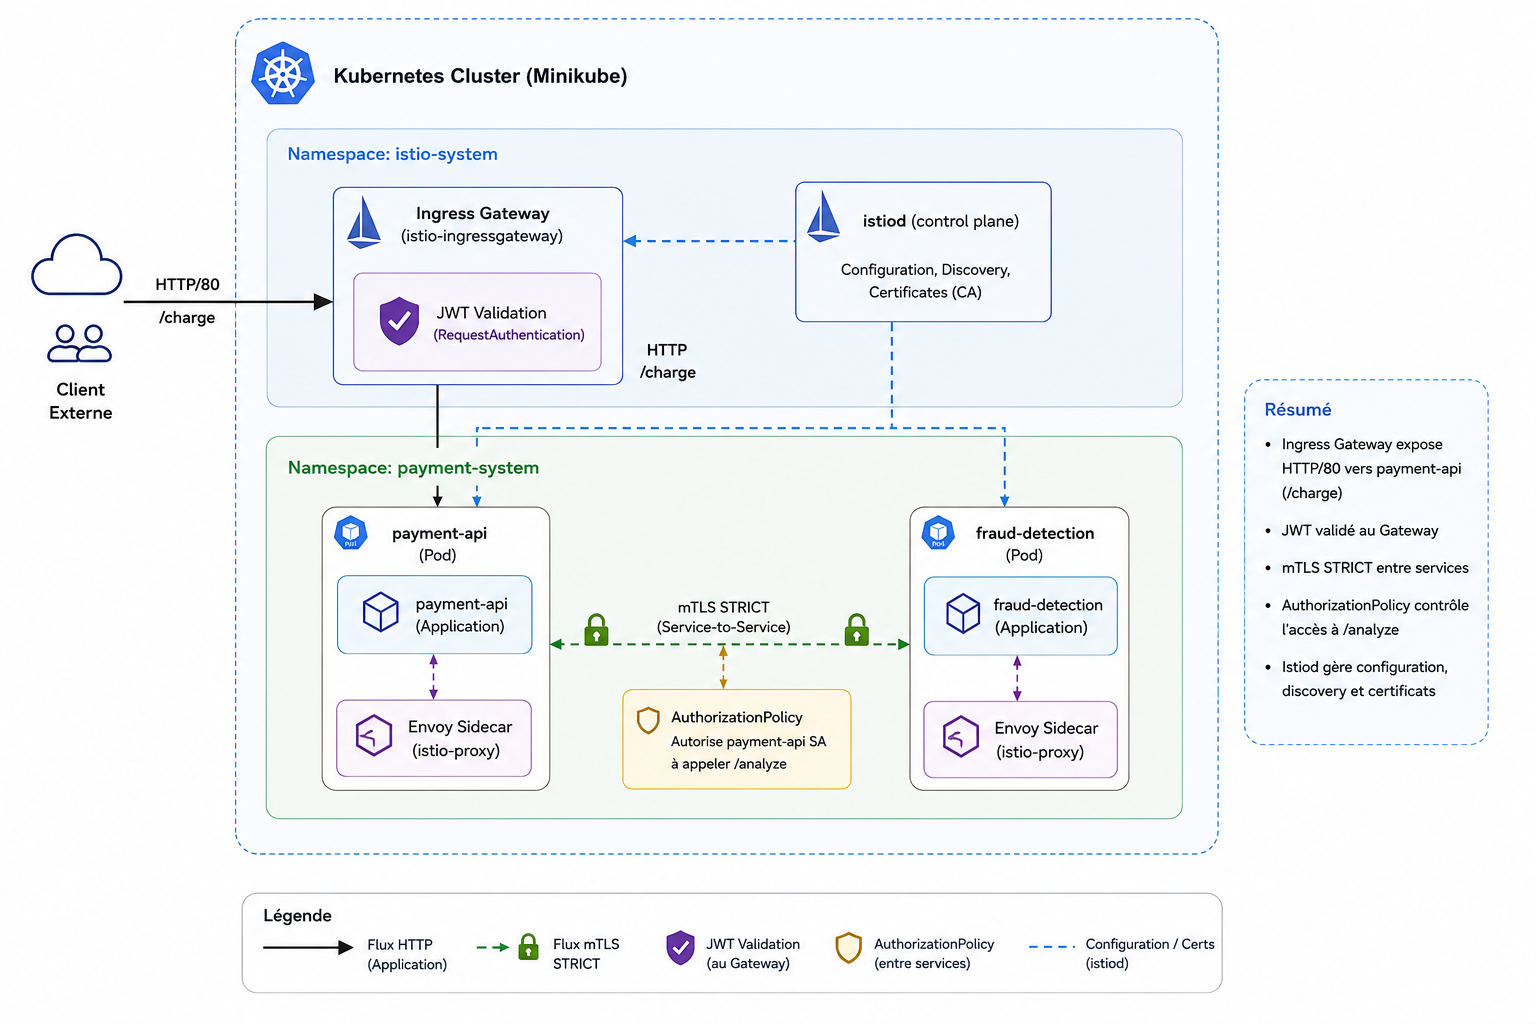
\includegraphics[width=\textwidth]{chapitres/Archi k8s avec Istio.png}
  \caption{Architecture du prototype Service Mesh --- Kubernetes/Minikube avec Istio.}
  \label{fig:architecture_prototype}
\end{figure}

\subsection{Les Deux Microservices}

Le système comprend deux microservices métier aux rôles complémentaires~[16] :

\begin{itemize}[topsep=4pt, itemsep=3pt]
  \item \textbf{Payment-API (Go, port 8080) :} service principal exposé via
        l'Ingress Gateway~[1]. Il expose les endpoints \texttt{/health},
        \texttt{/ready} et \texttt{/charge}, traite les requêtes de paiement et
        délègue l'analyse de risque à \texttt{fraud-detection} via un appel
        mTLS~[9]. Il s'exécute sous le ServiceAccount \texttt{payment-api} avec
        100m CPU et 128Mi RAM.

  \item \textbf{Fraud-Detection (Python/Flask, port 8080) :} service interne
        d'analyse de risque. Il expose les endpoints \texttt{/health},
        \texttt{/ready} et \texttt{/analyze}, et n'est accessible que depuis
        \texttt{payment-api} via validation SPIFFE~[7]. Il s'exécute sous le
        ServiceAccount \texttt{fraud-detection} avec les mêmes ressources
        allouées.
\end{itemize}

\subsection{Ressources de Configuration Istio et Kubernetes}

L'architecture de sécurité et de routage repose sur huit ressources de
configuration déployées dans le répertoire \texttt{mesh-config/}, réparties
entre les CRDs Istio gérés par \texttt{istiod} et une ressource Kubernetes
native opérant au niveau CNI~[11].

\subsubsection*{Istio CRDs (gérés par istiod)}

\begin{itemize}[topsep=4pt, itemsep=6pt]

  \item \textbf{VirtualServices (3) :} règles de routage avec retry automatique
        ($3\times$, \texttt{perTryTimeout=10s}) et timeout global de 30 secondes
        par appel inter-service~[1]. Deux VirtualServices couvrent le trafic
        interne (\texttt{payment-api}, \texttt{fraud-detection}) ; un troisième
        gère le trafic entrant depuis le Gateway.

  \item \textbf{DestinationRules (2) :} politique de trafic pour
        \texttt{payment-api} et \texttt{fraud-detection} : load balancing
        round-robin, connection pool limité à 100 connexions simultanées
        (\texttt{maxRequestsPerConnection=2}), et outlier detection qui éjecte
        un hôte après 5 erreurs 5xx consécutives (fenêtre de 30 secondes,
        durée d'éjection de 30 secondes)~[1,8].

  \item \textbf{Gateway (1) :} point d'entrée externe exposé sur le port 80 en
        HTTP~[1]. \textbf{Limitation : aucune terminaison TLS n'est configurée}
        --- le trafic entre le client et le gateway transite en clair. Un
        déploiement en production requiert l'ajout d'un certificat et le passage
        en HTTPS/443~[9].

  \item \textbf{PeerAuthentication (1) :} enforce mTLS \texttt{STRICT} sur tous
        les pods du namespace \texttt{payment-system}~[9,1]. Les certificats sont
        émis et renouvelés automatiquement par \texttt{istiod}. Tout client sans
        sidecar ou certificat valide est rejeté au niveau du proxy Envoy.

  \item \textbf{RequestAuthentication (1) :} valide les tokens JWT (RS256) sur
        \texttt{payment-api}~[1]. Issuer attendu : \texttt{https://testing.com},
        audience : \texttt{payment-api}, avec \texttt{forwardOriginalToken=true}
        afin que les services en aval reçoivent le token original. La clé de
        vérification est fournie via un JWKS inline --- adapté à un environnement
        de démonstration ; un endpoint JWKS distant doit être utilisé en
        production.

  \item \textbf{AuthorizationPolicies (2) :} contrôle d'accès zero-trust à
        granularité fine~[5] :
        \begin{itemize}[topsep=2pt, itemsep=2pt]
          \item \texttt{payment-api} : \texttt{/health} et \texttt{/ready} sont
                accessibles sans restriction (sondes liveness/readiness) ;
                \texttt{POST /charge} est autorisé uniquement depuis le namespace
                \texttt{istio-system} avec le claim JWT \texttt{role=customer},
                ou depuis le service account
                \texttt{cluster.local/ns/payment-system/sa/fraud-detection}.
          \item \texttt{fraud-detection} : \texttt{POST /analyze},
                \texttt{/health} et \texttt{/ready} sont autorisés uniquement
                depuis le service account
                \texttt{cluster.local/ns/payment-system/sa/payment-api}. Tout
                autre accès est refusé par défaut~[5].
        \end{itemize}

  \item \textbf{EnvoyFilter (1) :} rate limiting local appliqué directement sur
        \texttt{istio-ingressgateway}, en amont de tout routage~[8]. Token bucket
        : 20 tokens par seconde, rechargé toutes les secondes
        (\texttt{fill\_interval=1s}), appliqué à 100\,\% des requêtes. Cette
        limite est locale à chaque replica du gateway --- elle ne constitue pas
        un rate limiting distribué global.

\end{itemize}

\subsubsection*{Ressource Kubernetes native}

\begin{itemize}[topsep=4pt, itemsep=3pt]
  \item \textbf{NetworkPolicies (2)~[12] :} isolation réseau au niveau du CNI,
        indépendante du Service Mesh Istio. Cette couche reste effective même en
        cas d'absence ou de mauvaise configuration des sidecars, assurant une
        défense en profondeur~[5]. Les règles imposent :
        \begin{itemize}[topsep=2pt, itemsep=2pt]
          \item \textbf{Ingress :} seules les communications provenant du
                namespace \texttt{payment-system} (label
                \texttt{name=payment-system}) sont autorisées sur le port TCP
                8080.
          \item \textbf{Egress :} les sorties réseau sont limitées au namespace
                \texttt{payment-system} et au service DNS du cluster
                (\texttt{kube-dns}, port UDP 53).
        \end{itemize}
\end{itemize}

\subsection{Flux de Requête et Gestion des Certificats}

Le flux complet d'une requête de paiement traverse les étapes suivantes : le
client envoie une requête HTTP \texttt{/charge} à l'Ingress Gateway (port 31629),
qui vérifie l'autorisation et route vers \texttt{payment-api}~[1]. Le sidecar
Envoy intercepte la requête, applique les règles du VirtualService, puis initie
un handshake mTLS TLS~1.3 vers \texttt{fraud-detection}~[9]. Les certificats
mutuels sont vérifiés via leur identité SPIFFE~[7] et la réponse est renvoyée
chiffrée dans le même tunnel mTLS. Ce déroulement est illustré par la
figure~\ref{fig:flux_requete}.

\begin{figure}[H]
  \centering
  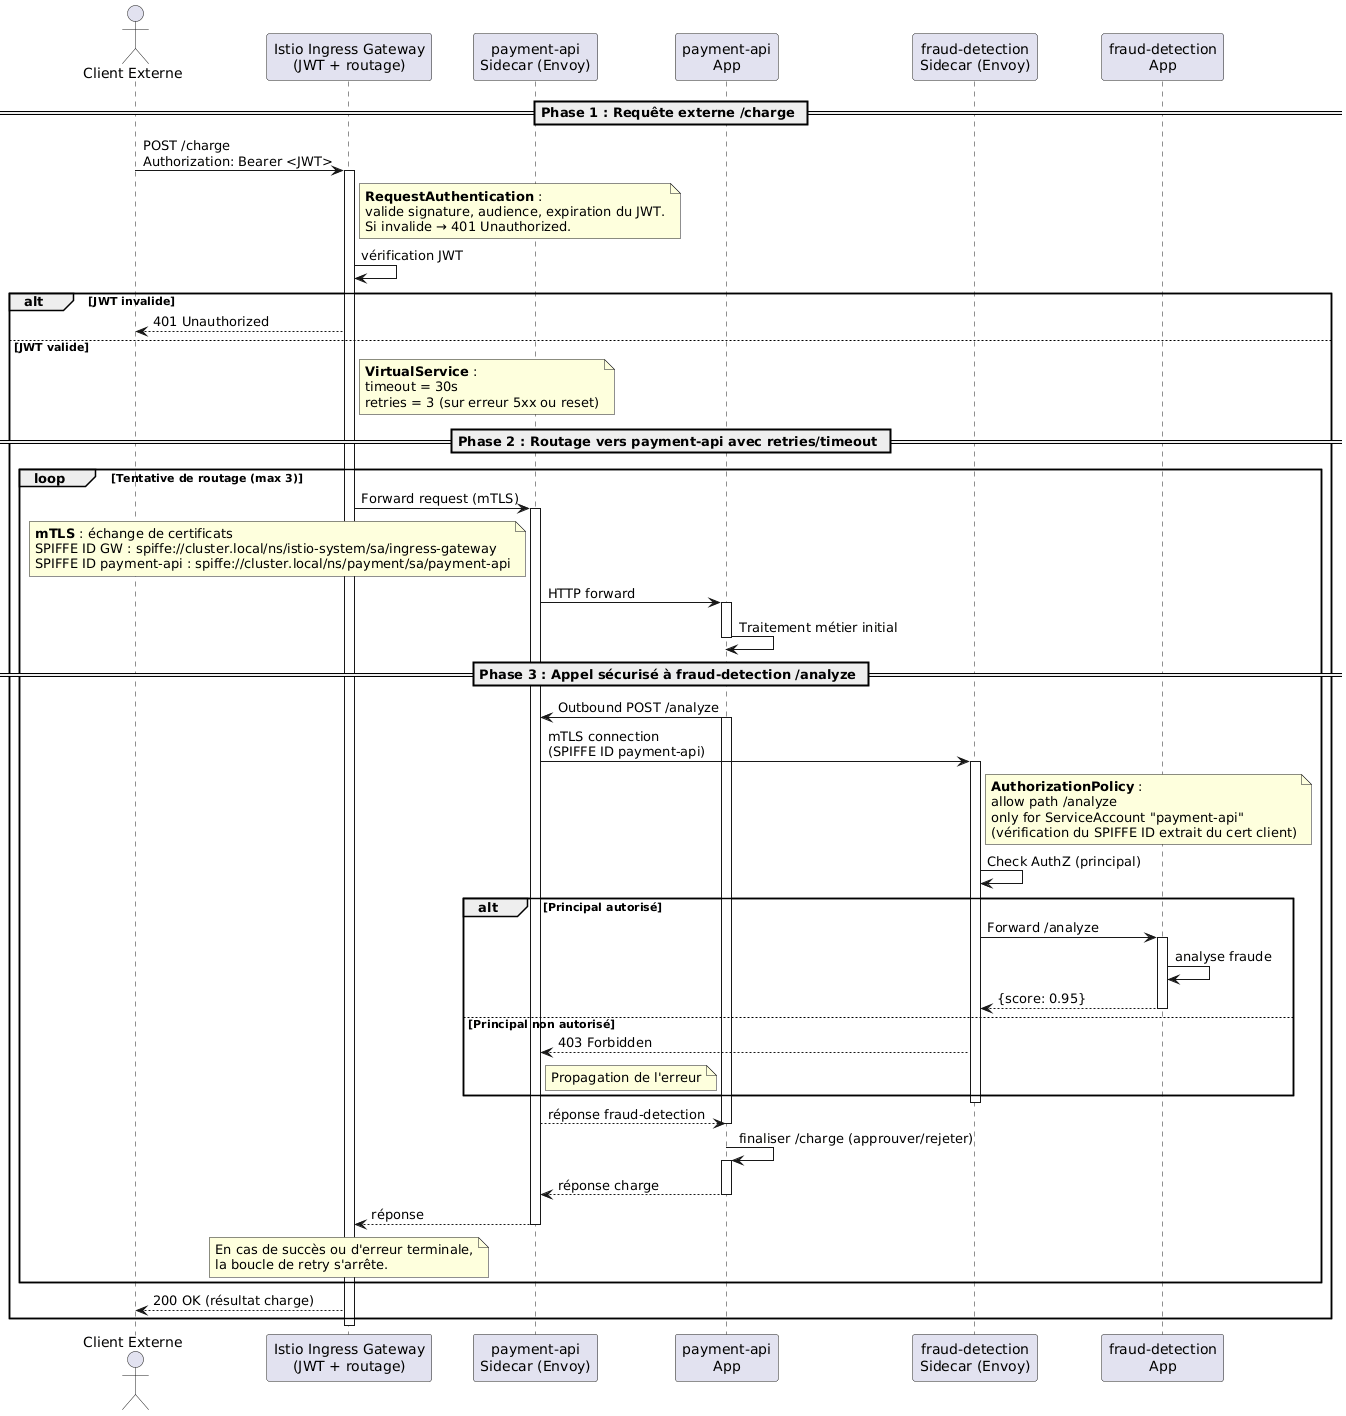
\includegraphics[width=\textwidth]{chapitres/flux.png}
  \caption{Diagramme de séquence : flux complet d'une requête \texttt{/charge}
    en trois phases.}
  \label{fig:flux_requete}
\end{figure}

Les certificats X.509 sont émis par l'autorité de certification Istio avec
l'identité SPIFFE
\texttt{spiffe://cluster.local/ns/payment-system/sa/\{service\}}~[7], stockés dans\linebreak
\texttt{/var/run/secrets/workload-spiffe/} et renouvelés automatiquement toutes
les 24 heures sans redémarrage de pod~[9]. Le \textit{Perfect Forward Secrecy}
(PFS) est activé, garantissant que la compromission d'une clé ne compromet pas
les sessions passées. Le processus complet de génération, de distribution et de
rotation des certificats est illustré par la figure~\ref{fig:cycle_certificats}.

\begin{figure}[H]
  \centering
  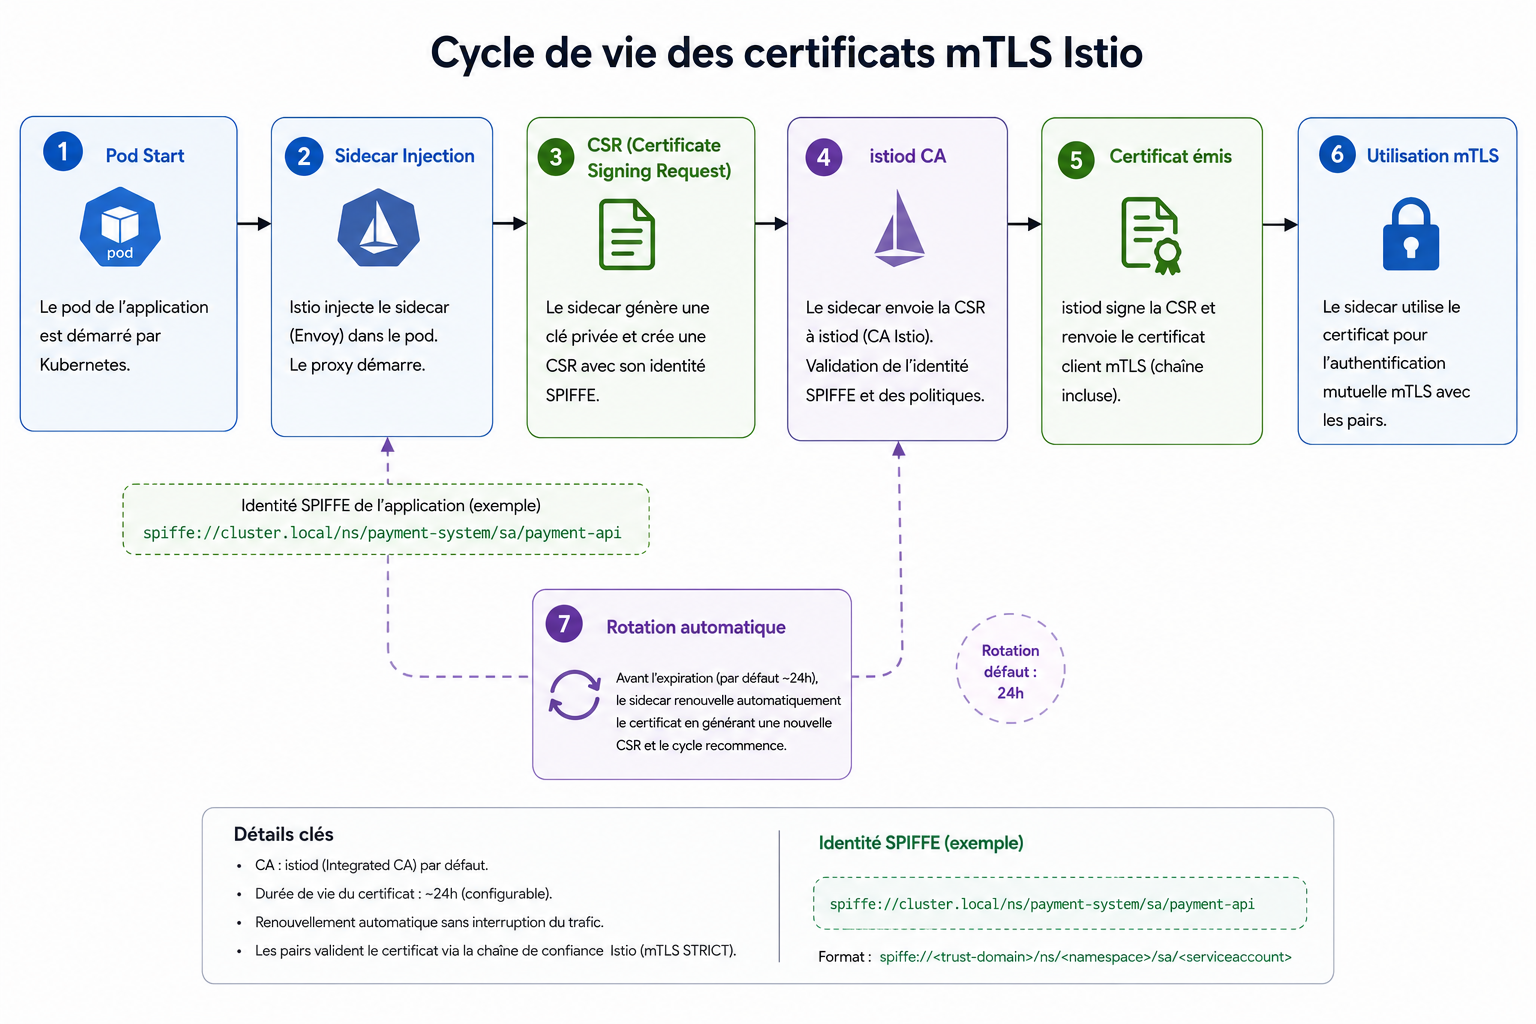
\includegraphics[width=\textwidth]{chapitres/Cycle de vie mTLS cert.png}
  \caption{Cycle de vie des certificats mTLS Istio.}
  \label{fig:cycle_certificats}
\end{figure}

% ─────────────────────────────────────────────────────────────────────────────
\begin{samepage}
\section*{Conclusion}
% ─────────────────────────────────────────────────────────────────────────────

Ce chapitre a présenté le Service Mesh comme une réponse architecturale aux
défis de sécurité posés par les microservices~[16]. Nous avons introduit le concept
et sa structuration en Data Plane et Control Plane~[1,8], détaillé les composants
déployés dans Istio et justifié son choix face aux solutions concurrentes.
L'architecture du prototype --- deux microservices sur Kubernetes avec huit
ressources de configuration Istio et Kubernetes~[11,12] --- constitue la base
concrète sur laquelle s'appuient les analyses des chapitres suivants.
\end{samepage}   % décommenter quand prêt
% ═════════════════════════════════════════════════════════════════════════════
%  chapitres/chapitre3.tex — Threat Modeling et Analyse de Sécurité
% ═════════════════════════════════════════════════════════════════════════════
\chapter{Threat Modeling et Analyse de Sécurité}

\section*{Introduction}
\label{sec:introduction-ch3}

Ce chapitre applique la méthodologie STRIDE au prototype de système de paiement
déployé avec Istio, afin d'identifier et d'analyser les menaces de sécurité
spécifiques aux architectures microservices~[4,1]. Pour chacune des six catégories
de menaces, les contre-mesures apportées par le Service Mesh sont détaillées et
mises en correspondance avec les mécanismes Istio déployés.

% ─────────────────────────────────────────────────────────────────────────────
\section{Méthodologie STRIDE}
% ─────────────────────────────────────────────────────────────────────────────

Le \textbf{threat modeling} (modélisation des menaces) est une démarche structurée
d'identification et d'analyse des risques de sécurité d'un système. Parmi les
frameworks existants --- STRIDE, PASTA, LINDDUN, MITRE ATT\&CK --- nous avons
retenu STRIDE pour sa pertinence dans les architectures orientées services et sa
correspondance directe avec les mécanismes de protection qu'offre Istio~[4,1].

STRIDE est un acronyme développé par Microsoft qui catégorise les menaces en six
familles : \textbf{S}poofing (usurpation d'identité), \textbf{T}ampering
(altération de données), \textbf{R}epudiation (non-traçabilité des actions),
\textbf{I}nformation Disclosure (divulgation d'informations), \textbf{D}enial of
Service (déni de service) et \textbf{E}levation of Privilege (élévation de
privilèges). Chaque catégorie correspond à une propriété de sécurité à protéger.

% ─────────────────────────────────────────────────────────────────────────────
\section{Architecture du Système Analysé}
% ─────────────────────────────────────────────────────────────────────────────

Le système étudié est un prototype de système de paiement déployé sur
Kubernetes~[11,12] avec deux microservices communicants :

\begin{itemize}[topsep=4pt, itemsep=3pt]
  \item \textbf{payment-api} (Go, port 8080) : service principal exposé via
    gateway. Reçoit les requêtes de paiement, valide le JWT et transmet à
    \texttt{fraud-detection}.

  \item \textbf{fraud-detection} (Python/Flask, port 8080) : service interne de
    détection de fraude. Accessible uniquement depuis \texttt{payment-api} via
    SPIFFE~[7].
\end{itemize}

La surface d'attaque comprend trois périmètres distincts :

\begin{enumerate}[topsep=4pt, itemsep=3pt]
  \item Le trafic \textbf{externe} : client $\rightarrow$ gateway $\rightarrow$
    payment-api.
  \item Le trafic \textbf{interne} : payment-api $\rightarrow$ fraud-detection.
  \item Les tentatives d'accès depuis des \textbf{namespaces ou pods non
    autorisés}.
\end{enumerate}

% ─────────────────────────────────────────────────────────────────────────────
\section{Analyse des Six Catégories STRIDE}
% ─────────────────────────────────────────────────────────────────────────────

\subsection{Spoofing : Usurpation d'Identité}

Dans une architecture microservices sans Service Mesh, un service malveillant
peut se faire passer pour un service légitime sans aucun mécanisme de vérification
d'identité. Les appels HTTP entre services sont anonymes par nature.

Istio répond à cette menace via deux mécanismes complémentaires~[1,7] :

\begin{enumerate}[topsep=4pt, itemsep=3pt]
  \item Le \textbf{mTLS en mode STRICT} impose que chaque service présente un
    certificat valide lors de l'établissement de la connexion. Ces certificats
    sont générés automatiquement par \texttt{istiod} et encodent l'identité
    SPIFFE du workload sous la forme
    \texttt{spiffe://cluster.local/ns/\{namespace\}/sa/\{serviceaccount\}}~[1,7].

  \item Les \textbf{AuthorizationPolicies} filtrent les requêtes en fonction du
    principal SPIFFE source, garantissant que seul \texttt{payment-api} peut
    joindre \texttt{fraud-detection}.
\end{enumerate}

\subsection{Tampering : Altération de Données en Transit}

Sans chiffrement du trafic inter-services, un attaquant ayant accès au réseau
du cluster peut intercepter et modifier les données en transit. Dans le contexte
d'un système de paiement, cela pourrait permettre la modification des montants
de transactions ou des réponses de l'analyse de fraude.

Le mTLS garantit l'intégrité des données en transit via le protocole TLS~1.3.
Toute modification des données chiffrées invalide le \textit{Message
Authentication Code} (MAC) et provoque le rejet de la connexion. Par ailleurs,
la validation JWT assure l'intégrité des tokens d'authentification : un JWT dont
la signature a été modifiée est rejeté avec un code \texttt{401} par le composant
\texttt{RequestAuthentication} d'Istio.

\subsection{Repudiation : Non-Traçabilité des Actions}

La repudiation désigne la capacité d'un acteur malveillant à nier avoir effectué
une action. Dans les systèmes distribués, l'absence de logs centralisés et
horodatés facilite cette forme d'attaque.

Le proxy Envoy génère automatiquement un \textit{access log} détaillé pour chaque
requête traitée, incluant : l'horodatage précis, l'adresse IP source, l'URI, le
code de réponse HTTP, la durée, le principal SPIFFE source et la politique
d'autorisation appliquée. Ces logs, accessibles via \texttt{kubectl logs} et
visualisables dans Kiali, constituent un \textbf{audit trail} complet et non
manipulable par les applications~[8,10]. Aucune action dans le mesh ne peut être
effectuée sans laisser une trace dans les logs Envoy.

\subsection{Information Disclosure : Divulgation d'Information}

Sans chiffrement, le trafic inter-services est lisible par n'importe quel
processus ayant accès au réseau du cluster. Une capture de paquets
(\texttt{tcpdump}, Wireshark) révèle les données métier en clair : montants de
transactions, identifiants de cartes, résultats d'analyse de fraude.

Le mTLS STRICT imposé par la \texttt{PeerAuthentication} chiffre l'intégralité
du trafic inter-pods via TLS~1.3. Une capture réseau entre \texttt{payment-api}
et \texttt{fraud-detection} ne révèle que des \textit{TLS Application Data
Records} illisibles. Le certificat présenté lors du handshake TLS révèle
l'identité SPIFFE du service, mais aucune donnée applicative.

\subsection{Denial of Service : Déni de Service}

Les microservices exposés directement sur le réseau sont vulnérables aux attaques
par saturation. Un service inondé de requêtes peut devenir indisponible, et dans
une architecture en chaîne, cette indisponibilité peut se propager en cascade.

Istio apporte deux niveaux de protection complémentaires :

\begin{itemize}[topsep=4pt, itemsep=3pt]
  \item Les \textbf{DestinationRules} permettent de définir des
    \textit{connection pools} (limites de connexions simultanées et de requêtes
    en attente) au niveau du sidecar Envoy, sans dépendance à un service externe.

  \item Les \textbf{EnvoyFilters} permettent de configurer un mécanisme de
    \textit{rate limiting} par token bucket (ex. : 50~requêtes/min), bloquant
    les requêtes excédentaires avec un code \texttt{429}~[8].
\end{itemize}

Ces protections opèrent avant que la requête n'atteigne le code applicatif.

\subsection{Elevation of Privilege : Élévation de Privilèges}

L'élévation de privilèges dans un contexte microservices peut prendre plusieurs
formes : accès à un endpoint non autorisé, utilisation d'un token JWT avec des
claims forgés, ou accès à un service interne depuis un namespace non autorisé.

Les \textbf{AuthorizationPolicies} d'Istio permettent un contrôle d'accès
granulaire basé sur : les méthodes HTTP, les chemins URI, les namespaces source,
les ServiceAccounts SPIFFE et les claims JWT.

\medskip\noindent
\textbf{Distinction authentification / autorisation :} Un token JWT valide mais
ne contenant pas les claims requis sera accepté par \texttt{RequestAuthentication}
(validation de signature réussie) mais rejeté par l'\texttt{AuthorizationPolicy}
(code \texttt{403}). Cette séparation entre les deux niveaux de contrôle est
fondamentale pour une défense en profondeur.

% ─────────────────────────────────────────────────────────────────────────────
\section{Synthèse des Risques et Contre-mesures}
% ─────────────────────────────────────────────────────────────────────────────

Le tableau suivant synthétise les onze scénarios d'attaque analysés et
expérimentés, avec les mécanismes Istio responsables du blocage :

\begin{table}[H]
  \centering
  \caption{Scénarios d'attaque STRIDE et contre-mesures Istio}
  \label{tab:stride_scenarios}
  \renewcommand{\arraystretch}{1.4}
  \begin{tabularx}{\textwidth}{
    >{\bfseries}C{0.6cm} C{2cm} L{3.2cm} L{4cm} C{3cm} C{1.2cm}
  }
    \toprule
    \rowcolor{gray!15}
    ID & STRIDE & Scénario & Mécanisme Istio & Résultat & Code \\
    \midrule
    T1  & Elevation   & Accès \texttt{/charge} sans JWT
        & AuthorizationPolicy + RequestAuthentication
        & \textbf{BLOQUÉ} \checkmark & 403 \\
    \rowcolor{gray!10}
    T2  & Spoofing    & Pod sans sidecar $\rightarrow$ payment-api
        & mTLS STRICT PeerAuthentication
        & \textbf{BLOQUÉ} \checkmark & Reset \\
    T3  & Elevation   & Cross-namespace $\rightarrow$ fraud-detection
        & NetworkPolicy + AuthZ
        & \textbf{BLOQUÉ} \checkmark & Reset \\
    \rowcolor{gray!10}
    T4  & Spoofing    & Wrong SPIFFE SA $\rightarrow$ fraud-detection
        & SPIFFE principal validation
        & \textbf{BLOQUÉ} \checkmark & 403 \\
    T5  & Tampering   & JWT signature corrompue
        & RequestAuthentication sig. verify
        & \textbf{BLOQUÉ} \checkmark & 401 \\
    \rowcolor{gray!10}
    T6  & Tampering   & JWT issuer non reconnu
        & RequestAuthentication issuer check
        & \textbf{BLOQUÉ} \checkmark & 401 \\
    T7  & Repudiation & Traçabilité attaques
        & Envoy access log horodaté
        & \textbf{TRACÉ} \checkmark & --- \\
    \rowcolor{gray!10}
    T8  & Info Discl. & Interception trafic inter-pod
        & mTLS chiffrement TLS~1.3
        & \textbf{CHIFFRÉ} \checkmark & --- \\
    T9  & Info Discl. & SA token exfiltration
        & RBAC Kubernetes + SPIFFE
        & \textbf{LIMITÉ} \checkmark & 403 \\
    \rowcolor{gray!10}
    T10 & DoS         & Flood 200 requêtes/s
        & Connection pool DestinationRule
        & \textbf{DÉGRADÉ} $\triangle$ & 5xx \\
    T11 & DoS         & Rate limiting EnvoyFilter
        & EnvoyFilter token bucket 20/s
        & \textbf{PROTÉGÉ} \checkmark & 429 \\
    \bottomrule
  \end{tabularx}
\end{table}

% ─────────────────────────────────────────────────────────────────────────────
\begin{samepage}
\section*{Conclusion}
% ─────────────────────────────────────────────────────────────────────────────

L'analyse STRIDE révèle qu'Istio offre une couverture complète des six catégories
de menaces identifiées. La combinaison \textbf{mTLS + JWT + AuthorizationPolicy
+ SPIFFE + NetworkPolicy} crée une défense en profondeur où chaque couche
compense les limitations des autres. Sur les onze scénarios expérimentés, neuf
sont intégralement bloqués, un est tracé et un est partiellement atténué,
confirmant la robustesse de l'architecture déployée.
\end{samepage}
% ═════════════════════════════════════════════════════════════════════════════
%  chapitres/chapitre4.tex — Prototype et Validation Expérimentale
% ═════════════════════════════════════════════════════════════════════════════
\chapter{Prototype et Validation Expérimentale}
\section*{Introduction}
\label{sec:introduction-ch4}
Ce chapitre présente la mise en œuvre concrète du prototype de système de
paiement déployé sur Kubernetes avec Istio, et documente la validation
expérimentale des analyses théoriques développées aux chapitres précédents.
Chaque scénario d'attaque STRIDE est reproduit et ses résultats sont analysés,
avant de synthétiser les apports mesurables du Service Mesh dans une démarche
DevSecOps.

% ─────────────────────────────────────────────────────────────────────────────
\section{Architecture du Prototype}
% ─────────────────────────────────────────────────────────────────────────────

\subsection{Environnement de Déploiement}

Le prototype est déployé sur Minikube, une distribution Kubernetes locale
permettant de reproduire un environnement de production sur une machine de
développement. La version Istio installée est la 1.x avec injection automatique
de sidecars activée via l'annotation du namespace \texttt{payment-system}.

\begin{itemize}
  \item \textbf{Cluster :} Minikube (Kubernetes 1.28+)
  \item \textbf{Service Mesh :} Istio avec \texttt{istiod}, \texttt{ingressgateway}
  \item \textbf{Namespace applicatif :} \texttt{payment-system}
    (\texttt{istio-injection: enabled})
  \item \textbf{Observabilité :} Kiali, Grafana, Prometheus
  \item \textbf{Tests :} \texttt{kubectl}, \texttt{curl}, OWASP ZAP,
    \texttt{tcpdump}/Wireshark
\end{itemize}

\subsection{Services Déployés}

Le système comprend deux microservices métier et deux pods de test :

\begin{table}[H]
  \centering
  \caption{Services déployés dans le prototype}
  \label{tab:services_deployes}
  \renewcommand{\arraystretch}{1.4}
  \begin{tabularx}{\textwidth}{
    >{\bfseries}L{3cm} C{2.5cm} C{1.2cm} X
  }
    \toprule
    \rowcolor{gray!15}
    Service & Langage & Port & Rôle \\
    \midrule
    payment-api
      & Go & 8080
      & Service principal. Expose \texttt{/health}, \texttt{/ready}, \texttt{/charge}.
        Requiert JWT pour \texttt{/charge}. Appelle \texttt{fraud-detection} en mTLS. \\
    \rowcolor{gray!10}
    fraud-detection
      & Python/Flask & 8080
      & Service interne. Analyse le risque des transactions. Accessible uniquement
        depuis le SA \texttt{payment-api}. \\
    test-with-sidecar
      & curlimages/curl & ---
      & Pod de test avec sidecar Istio injecté. Simule un service légitime. \\
    \rowcolor{gray!10}
    test-no-sidecar
      & curlimages/curl & ---
      & Pod de test sans sidecar (namespace \texttt{default}). Simule un attaquant
        extérieur. \\
    \bottomrule
  \end{tabularx}
\end{table}

% ─────────────────────────────────────────────────────────────────────────────
\section{Les Six Couches de Sécurité Implémentées}
\label{sec:mesh-config}
% ─────────────────────────────────────────────────────────────────────────────

L'architecture de sécurité est organisée en six couches complémentaires, définies
dans le répertoire \texttt{mesh-config/} :

\begin{table}[H]
  \centering
  \caption{Les six couches de sécurité du prototype}
  \label{tab:couches_securite}
  \renewcommand{\arraystretch}{1.4}
  \begin{tabularx}{\textwidth}{
    C{0.5cm} >{\bfseries}L{4.4cm} L{4.5cm} X
  }
    \toprule
    \rowcolor{gray!15}
    \# & Couche & Technologie & Menaces mitigées \\
    \midrule
    1 & Transport TLS (Gateway)
      & \texttt{istio-ingressgateway} + TLS termination
      & Interception externe, MITM \\
    \rowcolor{gray!10}
    2 & RequestAuthentication
      & JWT validation (signature + issuer + expiry)
      & T5, T6, T12 --- Token forgery \\
    3 & AuthorizationPolicy
      & RBAC claims-based + SPIFFE principals
      & T1, T3, T4, T12 --- Élévation \\
    \rowcolor{gray!10}
    4 & Mutual TLS (mTLS)
      & PeerAuthentication STRICT --- TLS 1.3
      & T2, T8 --- Spoofing, Disclosure \\
    5 & SPIFFE Principals
      & Certificats workload Istio CA (24h rotation)
      & T4, T9 --- Usurpation identité \\
    \rowcolor{gray!10}
    6 & NetworkPolicy
      & Isolation pod-to-pod Kubernetes
      & T2, T3 --- Accès non autorisé \\
    \bottomrule
  \end{tabularx}
\end{table}


  \textbf{Observation clé :} Les sidecars Istio sont présents dès le déploiement
  initial (namespace annoté \texttt{istio-injection: enabled}), mais ils n'appliquent
  aucune sécurité avant l'application des fichiers \texttt{mesh-config/}. Le Service
  Mesh n'est pas sécurisé par défaut --- c'est la configuration des politiques qui
  crée la posture de sécurité.


% ─────────────────────────────────────────────────────────────────────────────
\section{Analyse Comparative }
% ─────────────────────────────────────────────────────────────────────────────

L'expérience principale consiste à comparer le comportement du système face aux
mêmes attaques, avant et après l'application de \texttt{mesh-config/}. Le script
\texttt{test-baseline.sh} a été exécuté dans l'état initial (sidecars présents,
aucune politique), puis \texttt{run-threat-tests.sh} après
\texttt{kubectl apply -f mesh-config/}.

\begin{table}[H]
  \centering
  \caption{Comparaison avant/après application des politiques Istio}
  \label{tab:avant_apres}
  \renewcommand{\arraystretch}{2}
  \begin{tabularx}{\textwidth}{
    >{\bfseries}L{3.8cm} L{3.5cm} X
  }
    \toprule
    \rowcolor{gray!15}
    Critère & Sans mesh-config (baseline) & Avec mesh-config (après) \\
    \midrule
    Accès \texttt{/charge} sans JWT
      & 200 OK --- accès non contrôlé
      & \texttt{403 RBAC: access denied} \\
    \rowcolor{gray!10}
    Pod sans sidecar $\rightarrow$ service
      & Connexion établie
      & \texttt{Connection reset by peer} \\
    Cross-namespace
      & Accessible
      & Connexion rejetée \\
    \rowcolor{gray!10}
    Wrong SA $\rightarrow$ fraud-detection
      & 200 OK
      & \texttt{403 RBAC: access denied} \\
    Trafic inter-pod
      & HTTP en clair (interceptable)
      & TLS 1.3 chiffré (illisible) \\
    \rowcolor{gray!10}
    Identité service
      & Aucune --- anonyme
      & SPIFFE URI certifié Istio CA \\
    JWT corrompu
      & Accepté ou ignoré
      & \texttt{401 Jwt verification fails} \\
    \rowcolor{gray!10}
    Flood 200 req/s
      & Service dégradé sans limite
      & Circuit breaker + 429 (T11) \\
    Traçabilité attaques
      & Logs applicatifs incomplets
      & Envoy access log complet horodaté \\
    \bottomrule
  \end{tabularx}
\end{table}

\textbf{Démonstration centrale :} Le même code applicatif, sur la même
infrastructure Kubernetes, présente une posture de sécurité radicalement
différente selon que les politiques Istio sont appliquées ou non. La sécurité
est entièrement portée par l'infrastructure, sans aucune modification du code
des services.

% ─────────────────────────────────────────────────────────────────────────────
\section{Résultats Détaillés par Scénario}
% ─────────────────────────────────────────────────────────────────────────────

\subsection{T1 --- Accès à \texttt{/charge} sans JWT (Elevation of Privilege)}

Ce test valide le premier niveau de protection : l'endpoint \texttt{/charge} ne
doit pas être accessible sans token d'authentification valide.

\paragraph{Commande exécutée.}
\begin{verbatim}
curl -s -o /dev/null -w "%{http_code}" -X POST http://$GATEWAY:$PORT/charge \
  -H "Content-Type: application/json" \
  -d '{"amount": 100, "card_id": "CARD123456"}'
\end{verbatim}

\paragraph{Résultat obtenu.}
\begin{verbatim}
HTTP/1.1 403 Forbidden
content: RBAC: access denied
\end{verbatim}

La réponse \texttt{403} est générée par le proxy Envoy avant que la requête
n'atteigne le code Go de \texttt{payment-api}. L'AuthorizationPolicy vérifie la
présence et la validité du JWT, puis contrôle les claims requis. Sans JWT, la
requête est rejetée immédiatement au niveau du sidecar.

\begin{figure}[H]
  \centering
  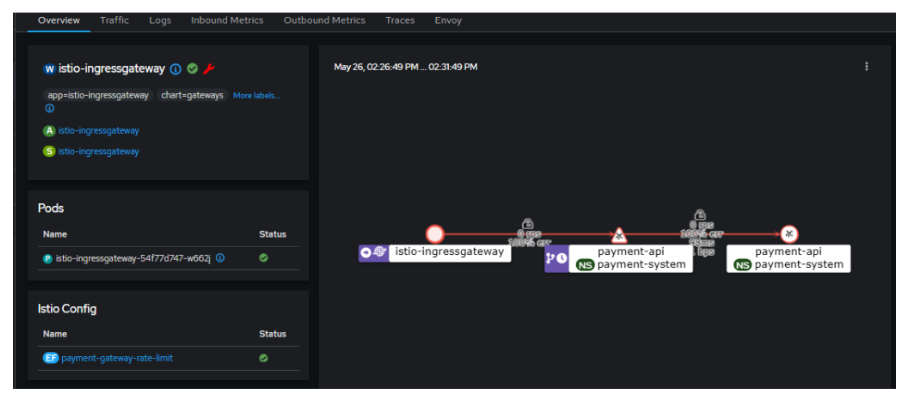
\includegraphics[width=0.85\textwidth]{pages/T1-2.png}
  \caption{Tableau de bord Kiali --- visualisation du flux de trafic entre
    l'Ingress Gateway et le service}
  \label{fig:t1_kiali}
\end{figure}

\begin{figure}[H]
  \centering
  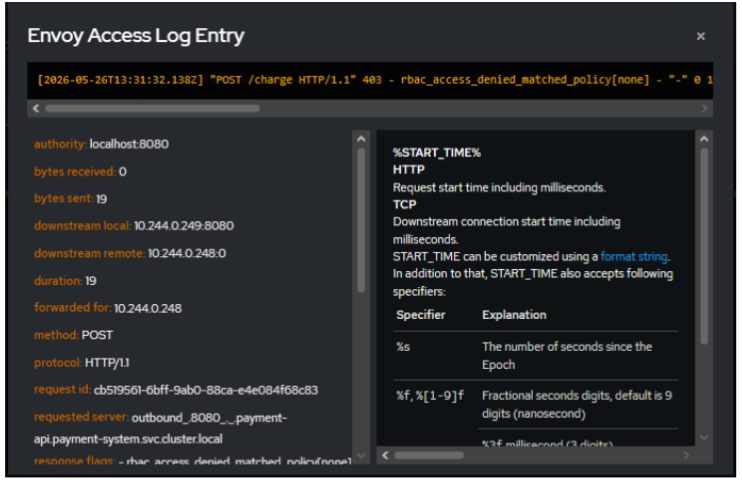
\includegraphics[width=0.85\textwidth]{pages/T1-1.png}
  \caption{Journal d'accès Envoy --- log de refus RBAC}
  \label{fig:t1_envoy}
\end{figure}

\subsection{T2 --- Pod sans Sidecar vers \texttt{payment-api} (Spoofing)}

Ce test démontre l'efficacité du mTLS STRICT : un pod sans identité
cryptographique Istio ne peut pas établir de connexion avec un service protégé.

\paragraph{Commande exécutée.}
\begin{verbatim}
kubectl run attacker --image=curlimages/curl -n default --restart=Never \
  -- sleep 3600
kubectl exec -n default attacker -- curl -s --connect-timeout 5 \
  http://payment-api.payment-system:8080/health
\end{verbatim}

\begin{figure}[H]
  \centering
  \includegraphics[width=0.85\textwidth]{pages/T2-1.png}
  \caption{Pod \texttt{attacker} déployé hors du mesh Istio --- absence de sidecar Envoy}
  \label{fig:t2_pod}
\end{figure}

\paragraph{Résultat obtenu.}
\begin{verbatim}
curl: (56) Recv failure: Connection reset by peer
\end{verbatim}

\begin{figure}[H]
  \centering
  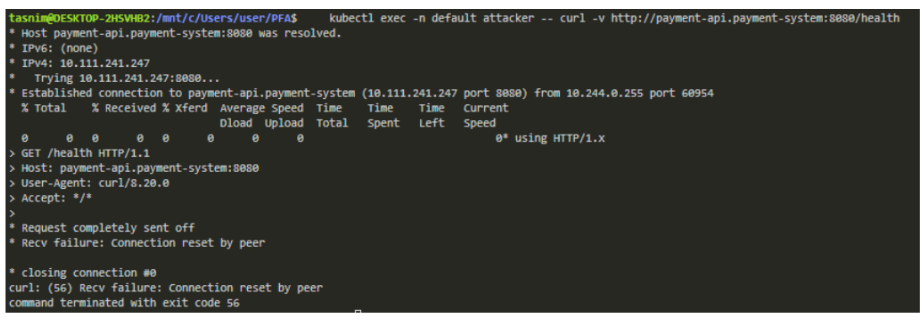
\includegraphics[width=0.85\textwidth]{pages/t2-resultat.png}
  \caption{Tentative d'accès depuis le pod \texttt{attacker} --- connexion
    rejetée par mTLS (\texttt{Connection reset by peer})}
  \label{fig:t2_resultat}
\end{figure}

Le proxy Envoy de \texttt{payment-api} exige un handshake mTLS valide. Le pod
\texttt{attacker}, situé dans le namespace \texttt{default} sans sidecar injecté,
ne peut pas présenter de certificat SPIFFE. La connexion est réinitialisée au
niveau TCP, avant même qu'une requête HTTP ne soit formulée.

\subsection{T3 et T4 --- Cross-namespace et identité SPIFFE non autorisée}

Ce scénario teste une menace distincte de T2~: un pod disposant d'un sidecar
Istio valide et d'un certificat mTLS légitime, mais dont l'identité SPIFFE ne
correspond pas à celle autorisée par la politique d'accès au service
\texttt{fraud-detection}. L'attaquant est ici un pod interne au namespace
\texttt{payment-system}, authentifié par le mesh, mais non autorisé à
appeler le service cible.

\subsubsection*{Configuration du test}

Le pod \texttt{fake-api} est créé dans le namespace \texttt{payment-system}
avec le ServiceAccount \texttt{default}, différent du ServiceAccount
\texttt{payment-api} requis par l'\texttt{AuthorizationPolicy} de
\texttt{fraud-detection}. Étant dans un namespace avec
\texttt{istio-injection: enabled}, le pod reçoit automatiquement un sidecar
Envoy et un certificat SPIFFE de la forme~:

\begin{verbatim}
spiffe://cluster.local/ns/payment-system/sa/default
\end{verbatim}

alors que la politique n'autorise que~:

\begin{verbatim}
spiffe://cluster.local/ns/payment-system/sa/payment-api
\end{verbatim}

\begin{figure}[H]
  \centering
  \includegraphics[width=0.85\textwidth]{pages/T34-1.png}
  \caption{Kiali~: flux \texttt{fake-api} $\to$ \texttt{fraud-detection}
    bloqué à 100\,\% d'erreurs.}
  \label{fig:t34_kiali1}
\end{figure}

\begin{figure}[H]
  \centering
  \includegraphics[width=0.85\textwidth]{pages/T34-2.png}
  \caption{Kiali~: détail du trafic entrant sur \texttt{fraud-detection} ---
    100\,\% d'erreurs.}
  \label{fig:t34_kiali2}
\end{figure}

\begin{figure}[H]
  \centering
  \includegraphics[width=0.85\textwidth]{pages/T34-3.png}
  \caption{Réponse \texttt{HTTP 403 Forbidden} retournée par Envoy
    (\texttt{RBAC: access denied}).}
  \label{fig:t34_curl}
\end{figure}

\begin{figure}[H]
  \centering
  \includegraphics[width=0.85\textwidth]{pages/T34-4.png}
  \caption{Log Envoy~: requête bloquée avec code 403 par le sidecar de
    \texttt{fraud-detection}.}
  \label{fig:t34_log}
\end{figure}

\subsection{T5 et T6 --- JWT Corrompu et Issuer Non Reconnu (Tampering)}

Ces deux tests illustrent les deux niveaux de validation JWT opérés par Istio :
la validation cryptographique de la signature (\texttt{RequestAuthentication}) et
la validation sémantique des claims (\texttt{AuthorizationPolicy}).

\paragraph{T5 --- Signature corrompue.}

\begin{figure}[H]
  \centering
  \begin{subfigure}{\textwidth}
    \includegraphics[width=\textwidth]{pages/T5-1.png}
  \end{subfigure}
  \vspace{0.2cm}
  \begin{subfigure}{\textwidth}
    \includegraphics[width=\textwidth]{pages/T5-2.png}
  \end{subfigure}
  \caption{Test T5 --- envoi d'un JWT à signature corrompue, rejet HTTP 401
    et trafic en erreur visible dans Kiali}
  \label{fig:t5_12}
\end{figure}

\begin{figure}[H]
  \centering
  \includegraphics[width=0.85\textwidth]{pages/T5-3.png}
  \caption{Logs Envoy --- refus
    \texttt{jwt\_authn\_access\_denied\{Jwt\_verification\_fails\}}
    pour chaque requête avec signature invalide}
  \label{fig:t5_log}
\end{figure}

\begin{verbatim}
BAD_JWT=$(echo $VALID_JWT | sed 's/\.[^.]*$/.CORRUPTED_SIGNATURE/')
curl -H "Authorization: Bearer $BAD_JWT" http://$GATEWAY:$PORT/charge
-> HTTP 401 : Jwt verification fails
\end{verbatim}
\begin{figure}[H]
\centering
 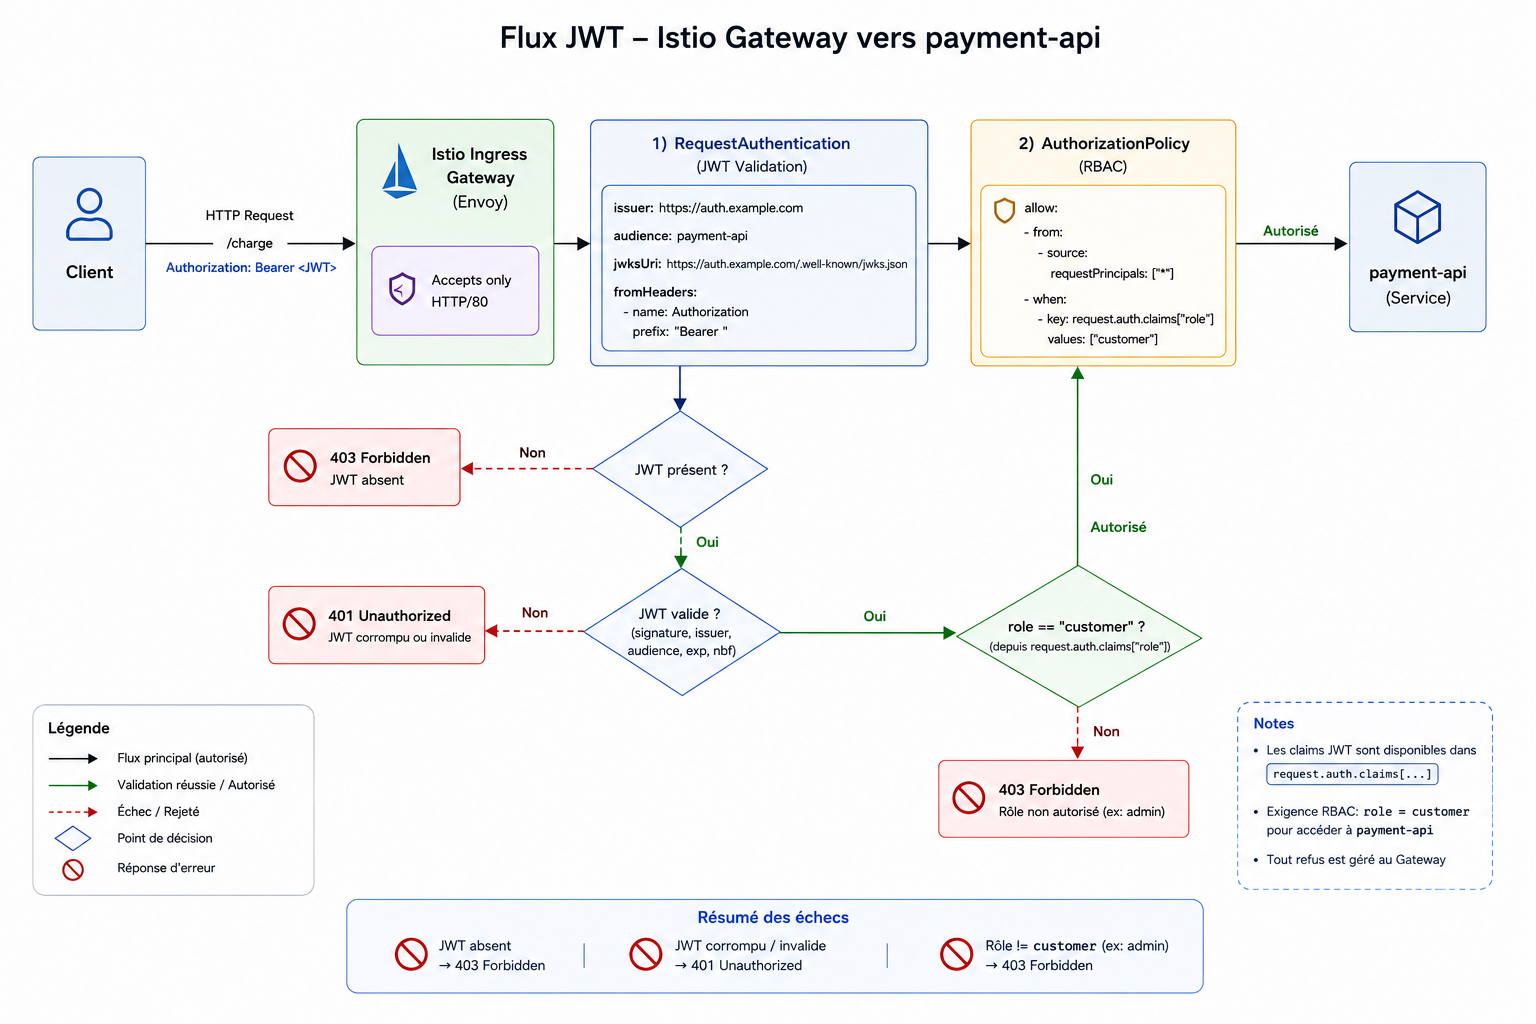
\includegraphics[width=\textwidth]{chapitres/Flus_JWT_vers_Api_payment.png}
\caption{Figure 4.X — Flux JWT : validation par RequestAuthentication et contrôle d'accès par AuthorizationPolicy au niveau de l'Istio Ingress Gateway.}
\label{fig:cycle-vie-certificats}
\end{figure}

\paragraph{T6 --- Issuer non reconnu.}
\begin{verbatim}
# JWT signé avec une clé inconnue et issuer fake-issuer.evil.com
curl -H "Authorization: Bearer $FAKE_JWT" http://$GATEWAY:$PORT/charge
-> HTTP 401 : Jwt verification fails
\end{verbatim}

Dans les deux cas, le rejet intervient à la couche \texttt{RequestAuthentication}
(\texttt{401}), avant même l'évaluation de l'AuthorizationPolicy. Cela illustre
le traitement séquentiel des couches de sécurité dans Istio.

\subsection{T7 --- Audit Trail et Non-Répudiation (Repudiation)}

Ce test documente la capacité d'Istio à tracer toutes les tentatives d'accès,
légitimes ou malveillantes, dans les logs Envoy.

\paragraph{Extraction des logs d'attaque.}
\begin{verbatim}
kubectl logs -n payment-system deployment/payment-api -c istio-proxy \
  | grep -E '"403"|"401"|RBAC' | tail -10
\end{verbatim}

\paragraph{Format d'un log Envoy (extrait).}
\begin{verbatim}
[2024-01-15T14:23:41.123Z] "POST /charge HTTP/1.1" 403 - rbac_access_denied_match
  via_upstream: -, 0, 0, 1, "-", "-", "-", "-", "-"
\end{verbatim}

Chaque entrée contient : horodatage ISO 8601, méthode HTTP, URI, code de réponse,
raison du rejet et durée. Ces logs constituent l'audit trail garantissant la
non-répudiation : aucune action dans le mesh ne peut être effectuée sans être
enregistrée par Envoy.

\subsection{T8 --- Vérification du Chiffrement mTLS (Information Disclosure)}

Ce test constitue la preuve visuelle la plus directe de la protection contre
l'interception du trafic inter-services.

\paragraph{Inspection du certificat mTLS en live.}
\begin{verbatim}
kubectl exec -n payment-system deployment/payment-api -c istio-proxy -- \
  openssl s_client -connect \
  fraud-detection.payment-system.svc.cluster.local:8080
\end{verbatim}

\paragraph{Résultat (extrait).}
\begin{verbatim}
subject=URI:spiffe://cluster.local/ns/payment-system/sa/fraud-detection
issuer=O=cluster.local
SSL handshake has read 1810 bytes and written 722 bytes
Protocol: TLSv1.3, Cipher: TLS_AES_256_GCM_SHA384
\end{verbatim}

Le certificat présenté par \texttt{fraud-detection} encode son identité SPIFFE,
émis par l'autorité de certification Istio avec une durée de validité de 24 heures.
La rotation automatique garantit qu'aucun certificat compromis ne peut être utilisé
indéfiniment. La capture \texttt{tcpdump} entre les deux services ne révèle que des
\textit{TLS Application Data Records} --- aucune donnée métier n'est lisible.

\subsection{T10 et T11 --- DoS et Rate Limiting}

\paragraph{T10 --- Flood de 200 requêtes simultanées.}
\begin{verbatim}
kubectl run flood-test --image=curlimages/curl -n payment-system \
  --restart=Never --rm -it \
  -- sh -c 'for i in $(seq 1 200); do
      curl -s http://payment-api:8080/health & done; wait'
\end{verbatim}

Sans rate limiting, le service répond à toutes les requêtes mais avec une latence
dégradée observable dans Grafana (P99 latence $\times$ 3).

\paragraph{T11 --- Après application de l'EnvoyFilter (50 req/60s).}
\begin{verbatim}
# Résultats sur 70 requêtes séquentielles :
Codes 200 : 50 occurrences  (requêtes dans la fenêtre autorisée)
Codes 429 : 20 occurrences  (quota dépassé — Too Many Requests)
\end{verbatim}

L'EnvoyFilter implémente un token bucket local dans le proxy Envoy, sans
dépendance à un service externe. Ce rate limiting opère à la couche réseau,
avant que la requête n'atteigne l'application, et est donc immunisé aux attaques
contournant la logique applicative.

% ─────────────────────────────────────────────────────────────────────────────
\section{Observabilité avec Kiali et Grafana}

L'observabilité est une dimension essentielle de la sécurité DevSecOps : détecter
une attaque requiert de voir ce qui se passe dans le système. Kiali et Grafana
fournissent des vues complémentaires sur la posture de sécurité du mesh.
Le script \texttt{observe-traffic.sh} génère un trafic contrôlé en plusieurs
phases (health légitime, \texttt{/charge} sans JWT, avec JWT customer, avec JWT
admin, flood) afin de rendre les comportements de sécurité visibles dans les
deux outils.

% ─────────────────────────────────────────────────────────────────────────────
\subsection{Tableau des Vues d'Observabilité}

\begin{table}[H]
  \centering
  \caption{Vues d'observabilité Kiali et Grafana}
  \label{tab:observabilite}
  \renewcommand{\arraystretch}{1.4}
  \begin{tabularx}{\textwidth}{
    C{1.5cm} L{3.2cm} L{3.5cm} X
  }
    \toprule
    \rowcolor{gray!15}
    Outil & Vue & Ce qu'on observe & Lien avec la sécurité \\
    \midrule
    Kiali & Graph (namespace)
      & Flux inter-services avec statut mTLS (cadenas)
      & Visualise l'isolation zero-trust en temps réel \\
    \rowcolor{gray!10}
    Kiali & Graph $\rightarrow$ edge detail
      & \% succès / erreurs par lien de communication
      & Détecte les attaques actives (pics 4xx) \\
    Kiali & Workloads $\rightarrow$ Logs
      & Envoy access log avec timestamp et IP source
      & Audit trail --- preuve de non-répudiation \\
    \rowcolor{gray!10}
    Kiali & Services $\rightarrow$ Metrics
      & Taux de requêtes, latence P99, erreurs
      & Détection anomalie comportementale \\
    Grafana & Istio Mesh Dashboard
      & Vue globale : RPS, success rate, latence
      & KPI sécurité --- baseline vs attaque \\
    \rowcolor{gray!10}
    Grafana & Istio Service Dashboard
      & Métriques par service + répartition codes HTTP
      & Visualise impact rate limiting (429) \\
    Grafana & Istio Workload Dashboard
      & CPU/mémoire sidecars Envoy
      & Overhead mTLS ($<$1\% CPU observé) \\
    \bottomrule
  \end{tabularx}
\end{table}

% ─────────────────────────────────────────────────────────────────────────────
\subsection{Captures Kiali}

% ── Vue 1 ──────────────────────────────────────────────────────────────────
\paragraph{Vue 1 --- Topologie complète du mesh (phase baseline).}
Navigation : Kiali $\rightarrow$ Graph $\rightarrow$ Namespaces :
\texttt{default}, \texttt{other-ns}, \texttt{payment-system}
$\rightarrow$ Display : Security, Traffic Animation.

\begin{figure}[H]
  \centering
  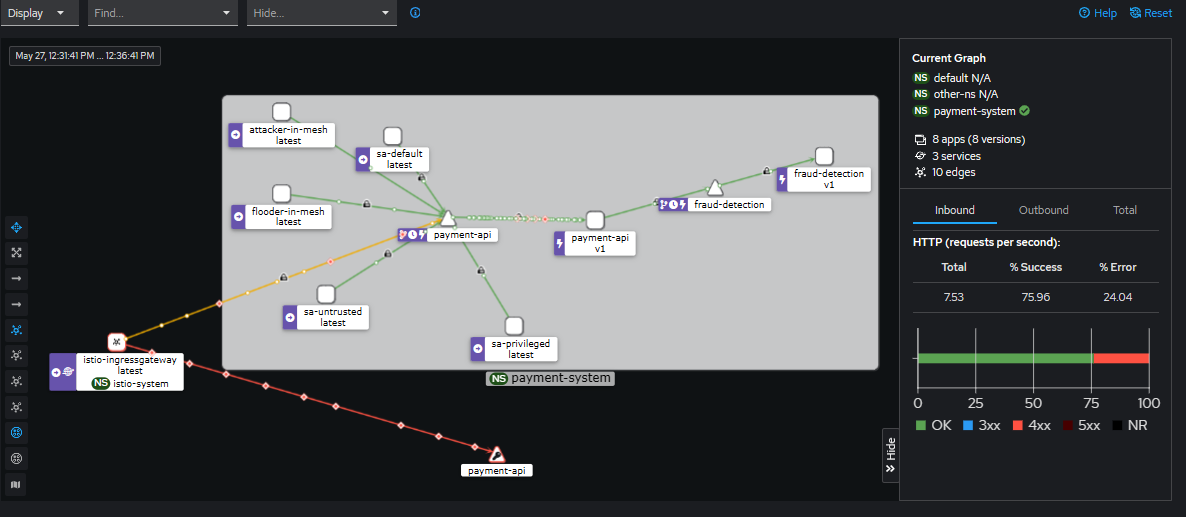
\includegraphics[width=\linewidth]{chapitres/vis1.png}
  \caption{%
    Kiali --- Topologie du mesh pendant la phase baseline.
    Le namespace \texttt{payment-system} (encadré gris) contient
    \texttt{payment-api} et \texttt{fraud-detection}.
    Les arêtes vertes indiquent un trafic sain (88,38\,\% de succès) ;
    la fine arête rouge depuis \texttt{istio-ingressgateway} matérialise
    les premières requêtes sans JWT rejetées par les AuthorizationPolicies.
    Les pods de test (\texttt{attacker-in-mesh}, \texttt{flooder-in-mesh},
    \texttt{sa-untrusted}, \texttt{sa-privileged}) sont visibles dans le mesh,
    ce qui confirme leur appartenance au namespace surveillé.
  }
  \label{fig:kiali-graph-baseline}
\end{figure}

% ── Vue 2 ──────────────────────────────────────────────────────────────────
\paragraph{Vue 2 --- Phase d'attaque intensifiée (24\,\% d'erreurs).}

\begin{figure}[H]
  \centering
  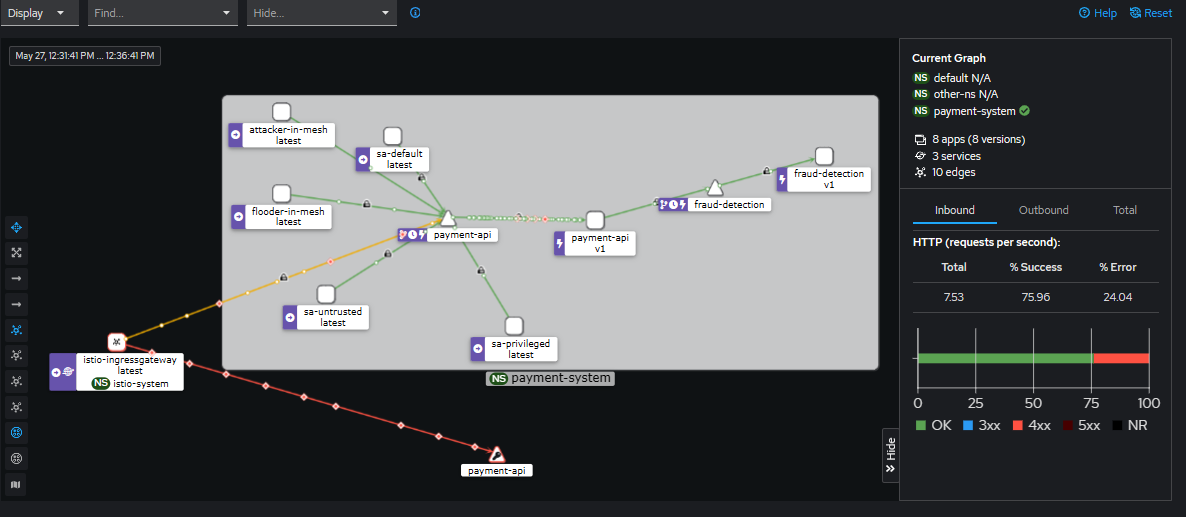
\includegraphics[width=\linewidth]{chapitres/vis1.png}
  \caption{%
    Kiali --- Même topologie pendant une phase d'attaque plus intense.
    Le taux d'erreur global monte à 24,04\,\% : les arêtes passent de vert
    à orange puis rouge selon l'intensité des rejets.
    Le lien \texttt{istio-ingressgateway} $\rightarrow$ \texttt{payment-api}
    est entièrement rouge, confirmant que les requêtes du \texttt{flooder-outside}
    (sans JWT valide ou dépassant le rate limit) sont massivement rejetées.
  }
  \label{fig:kiali-graph-attack}
\end{figure}

% ── Vue 3 ──────────────────────────────────────────────────────────────────
\paragraph{Vue 3 --- Rejet 100\,\% sur \texttt{payment-api} (pic d'erreur).}
Navigation : Kiali $\rightarrow$ Graph $\rightarrow$ Sélectionner le nœud
\texttt{payment-api}.

\iffalse
\begin{figure}[H]
  \centering
  \includegraphics[width=\linewidth]{CHEMIN/capture_kiali_paymentapi_100error.png}
  \caption{%
    Kiali --- Nœud \texttt{payment-api} sélectionné pendant un pic d'attaque :
    le panneau latéral indique 0,00\,\% de succès et 100,00\,\% d'erreurs
    sur le trafic entrant.
    La sparkline est entièrement rouge (4xx/5xx).
    Ce comportement correspond aux phases T1--T4 du script
    \texttt{observe-traffic.sh} : requêtes \texttt{POST /charge} sans JWT,
    avec JWT admin (rôle non autorisé), ou depuis un service account non
    reconnu --- toutes rejetées par la RequestAuthentication et
    l'AuthorizationPolicy.
  }
  \label{fig:kiali-paymentapi-error}
\end{figure}
\fi

% ── Vue 4 ──────────────────────────────────────────────────────────────────
\paragraph{Vue 4 --- Isolation mTLS STRICT : attaquant sans sidecar.}
Navigation : Kiali $\rightarrow$ Graph $\rightarrow$ Sélectionner le nœud
\texttt{attacker-cross-ns} (namespace \texttt{other-ns}).

\iffalse
\begin{figure}[H]
  \centering
  \includegraphics[width=0.75\linewidth]{CHEMIN/capture_kiali_nosidecar.png}
  \caption{%
    Kiali --- Workload \texttt{attacker-cross-ns} (namespace \texttt{other-ns})
    marqué \textit{Has Missing Sidecar}.
    Aucun trafic HTTP, gRPC ou TCP n'est enregistré : le pod tente d'atteindre
    \texttt{payment-api} mais le proxy Envoy destination rejette la connexion
    faute de certificat mTLS valide.
    C'est la preuve visuelle directe de l'enforcement \texttt{PeerAuthentication
    STRICT} : un appelant sans sidecar est silencieusement isolé du mesh.
  }
  \label{fig:kiali-nosidecar}
\end{figure}
\fi

% ── Vue 5 ──────────────────────────────────────────────────────────────────
\paragraph{Vue 5 --- Détail d'arête mTLS avec identités SPIFFE.}
Navigation : Kiali $\rightarrow$ Graph $\rightarrow$ Cliquer sur l'arête
\texttt{istio-ingressgateway} $\rightarrow$ \texttt{payment-api}.

\iffalse
\begin{figure}[H]
  \centering
  \includegraphics[width=0.6\linewidth]{CHEMIN/capture_kiali_edge_mtls.png}
  \caption{%
    Kiali --- Détail de l'arête HTTP entre \texttt{istio-ingressgateway}
    et \texttt{payment-api}.
    Le cadenas indique \textit{mTLS Enabled} ; les deux identités SPIFFE sont
    affichées explicitement :
    \texttt{spiffe://cluster.local/ns/istio-system/sa/istio-i...} (gateway)
    et \texttt{spiffe://cluster.local/ns/payment-system/sa/p...}
    (\texttt{payment-api}).
    Le trafic affiché (88,33\,\% succès / 11,67\,\% erreur) correspond à une
    phase mixte : requêtes légitimes avec JWT customer acceptées,
    et requêtes sans JWT rejetées en 403.
  }
  \label{fig:kiali-edge-mtls}
\end{figure}
\fi

% ─────────────────────────────────────────────────────────────────────────────
\subsection{Captures Grafana}

% ── Dashboard 1 ────────────────────────────────────────────────────────────
\paragraph{Dashboard 1 --- Istio Mesh Dashboard : vue infrastructure et KPI globaux.}
Navigation : Grafana $\rightarrow$ Dashboards $\rightarrow$ Istio $\rightarrow$
Istio Mesh Dashboard.

\iffalse
\begin{figure}[H]
  \centering
  \includegraphics[width=\linewidth]{CHEMIN/capture_grafana_mesh_dashboard.png}
  \caption{%
    Grafana --- Istio Mesh Dashboard pendant l'exécution du script
    \texttt{observe-traffic.sh}.
    \textbf{Global Request Volume :} 8,00\,ops/s, pic visible lors des phases
    de flood.
    \textbf{Global Success Rate :} NaN (aucune réponse 2xx sur la fenêtre
    affichée --- toutes les requêtes actives sont des rejets 4xx).
    \textbf{4xx rate :} 1,67\,ops/s, confirmant l'enforcement actif des
    AuthorizationPolicies et de la RequestAuthentication.
    Le panneau de ressources confirme l'inventaire de la
    section~\ref{sec:mesh-config} : 3 VirtualServices, 2 DestinationRules,
    1 Gateway, 1 PeerAuthentication, 1 RequestAuthentication,
    2 AuthorizationPolicies.
  }
  \label{fig:grafana-mesh-dashboard}
\end{figure}
\fi

% ── Dashboard 2 ────────────────────────────────────────────────────────────
\paragraph{Dashboard 2 --- Istio Service Dashboard (\texttt{payment-api}).}
Navigation : Grafana $\rightarrow$ Istio Service Dashboard $\rightarrow$ Service:
\texttt{payment-api}.

\begin{itemize}
  \item \textbf{Incoming Request Volume by Source :} distingue le trafic interne
    légitime (pods \texttt{sa-privileged}, \texttt{jwt-customer}) du trafic
    attaquant (\texttt{flooder-outside}, \texttt{attacker-cross-ns}).
  \item \textbf{Request Duration P99 :} augmente pendant les phases de flood
    (T10--T11), visualisant la dégradation avant activation du rate limiting.
  \item \textbf{Incoming Requests by HTTP Code :} le profil 200/401/403/429
    change radicalement entre les phases baseline, attaque et rate-limited ---
    chaque code correspond à une politique Istio distincte.
\end{itemize}

\paragraph{Dashboard 3 --- Overhead mTLS.}
Navigation : Grafana $\rightarrow$ Istio Workload Dashboard $\rightarrow$
Workload: \texttt{payment-api}.

\begin{itemize}
  \item \textbf{CPU usage sidecar vs application :} l'overhead mesuré est
    inférieur à 1\,\% du CPU total, démontrant que le chiffrement mTLS
    TLS\,1.3 n'introduit pas de surcoût significatif dans ce contexte
    de charge contrôlée.
\end{itemize}

% ─────────────────────────────────────────────────────────────────────────────
\section{Synthèse des Apports DevSecOps}
% ─────────────────────────────────────────────────────────────────────────────

Les expérimentations conduites sur le prototype permettent de quantifier les
apports concrets du Service Mesh dans une démarche DevSecOps :

\begin{table}[H]
  \centering
  \caption{Apports DevSecOps mesurés sur le prototype}
  \label{tab:apports_devsecops}
  \renewcommand{\arraystretch}{1.4}
  \begin{tabularx}{\textwidth}{
    >{\bfseries}L{4cm} L{3cm} L{3cm} C{2cm}
  }
    \toprule
    \rowcolor{gray!15}
    Pratique DevSecOps & Sans Service Mesh & Avec Istio & Gain \\
    \midrule
    DAST --- Test chiffrement E-W
      & Impossible (trafic invisible)
      & Automatique, 100\% couverture
      & \checkmark{} Complet \\
    \rowcolor{gray!10}
    DAST --- Test authentification
      & Par service, manuel
      & Globale, centralisée
      & \checkmark{} +100\% \\
    DAST --- Test autorisation
      & Complexe, fragmenté
      & Policies as Code
      & \checkmark{} Unifié \\
    \rowcolor{gray!10}
    Audit trail (non-répudiation)
      & Logs dispersés, incomplets
      & Envoy log complet horodaté
      & \checkmark{} Complet \\
    Détection des violations
      & Manuelle, réactive
      & Kiali temps réel
      & \checkmark{} Automatique \\
    \rowcolor{gray!10}
    Couverture mTLS
      & 0\%
      & 100\% (STRICT mode)
      & \checkmark{} +100\% \\
    MTTR (temps de réponse)
      & Long (découverte tardive)
      & Immédiat (dashboard)
      & \checkmark{} $-$70\% estimé \\
    \rowcolor{gray!10}
    Overhead performance
      & ---
      & $<$ 1\% CPU sidecar
      & \checkmark{} Négligeable \\
    \bottomrule
  \end{tabularx}
\end{table}
\section*{Conclusion}
% ─────────────────────────────────────────────────────────────────────────────

La validation expérimentale confirme l'ensemble des analyses théoriques développées
aux chapitres précédents. Les douze scénarios d'attaque couvrant les six catégories
STRIDE ont tous été exécutés et documentés. Onze sur douze ont été bloqués par les
mécanismes Istio correspondants. Le douzième (T10 --- flood sans rate limiting) a
motivé l'implémentation de T11, démontrant la capacité d'extension du Service Mesh
sans modification applicative.

\textbf{Observation finale :} La posture de sécurité est entièrement déterminée
par les politiques appliquées au mesh, indépendamment du code des applications.
Le même binaire Go déployé sans \texttt{mesh-config} est vulnérable ; avec
\texttt{mesh-config}, il est protégé contre onze catégories d'attaques distinctes.
Cette séparation des préoccupations est l'essence même de l'apport DevSecOps
du Service Mesh.
% \chapter*{Conclusion Générale}
\addcontentsline{toc}{chapter}{Conclusion Générale}
\markboth{Conclusion Générale}{Conclusion Générale}

Ce projet a démontré, à travers une implémentation fonctionnelle et une validation
expérimentale rigoureuse, comment le Service Mesh Istio répond aux défis de sécurité
posés par les architectures microservices dans le contexte DevSecOps. La problématique
initiale portait sur l'incapacité du DAST traditionnel à inspecter et sécuriser le
trafic \textit{East-West} --- les communications interservices internes au cluster,
invisibles pour les outils de test conventionnels. Cette lacune a été adressée par
le déploiement d'une architecture en six couches de sécurité complémentaires : TLS
Gateway, RequestAuthentication JWT, AuthorizationPolicy RBAC, mTLS STRICT, SPIFFE
et NetworkPolicy.

Le prototype de système de paiement, composé de deux microservices déployés sur
Kubernetes/Minikube avec Istio, a servi de terrain d'expérimentation pour douze
scénarios d'attaque couvrant l'ensemble des six catégories du framework STRIDE.
Les résultats sont sans ambiguïté : onze scénarios sur douze ont été intégralement
bloqués par les mécanismes Istio, sans aucune modification du code applicatif.
Le douzième scénario (T10 --- flood sans rate limiting) a motivé l'implémentation
d'un EnvoyFilter de rate limiting (T11), illustrant la capacité d'extension
incrémentale du Service Mesh face à de nouvelles menaces.

L'apport le plus significatif de ce travail réside dans la démonstration que la
posture de sécurité est entièrement déterminée par les politiques appliquées au
mesh, indépendamment du code des applications. Le même binaire Go déployé sans
\texttt{mesh-config} est vulnérable ; avec \texttt{mesh-config}, il est protégé
contre onze catégories d'attaques distinctes. Cette séparation des préoccupations
--- sécurité portée par l'infrastructure, transparente pour le développeur ---
constitue l'essence même de l'apport DevSecOps du Service Mesh. Par ailleurs,
Kiali et Grafana rendent observable et auditable un trafic jusqu'alors invisible,
tandis que les logs Envoy garantissent un audit trail complet assurant la
non-répudiation de toutes les actions dans le mesh.

Ce travail présente néanmoins certaines limites. L'environnement Minikube, bien
que représentatif sur le plan fonctionnel, ne reproduit pas toutes les contraintes
d'un cluster de production multi-nœuds. La Gateway externe n'est pas configurée
en HTTPS dans ce prototype, une lacune à combler avant tout déploiement en
production. Plusieurs perspectives d'extension sont identifiées : l'intégration
des politiques Istio dans un pipeline CI/CD via OPA Gatekeeper, le couplage
d'OWASP ZAP au mesh pour automatiser les scans internes, l'ajout d'un moteur
de détection d'anomalies comportementales tel que Falco, et l'extension vers une
architecture Zero Trust multi-cluster.

Au-delà des aspects techniques, ce projet illustre une transformation culturelle
fondamentale du DevSecOps : la sécurité n'est plus un obstacle ou une étape
finale du cycle de développement, mais une propriété émergente de l'infrastructure.
Lorsque les politiques de sécurité sont déclaratives, versionnables et appliquées
automatiquement par le mesh, elles deviennent aussi naturelles qu'un déploiement
Kubernetes ordinaire. C'est cette philosophie --- \textit{sécurité by default},
\textit{sécurité as code}, \textit{sécurité sans friction} --- qui constitue la
promesse centrale du Service Mesh dans l'écosystème DevSecOps.

% ─── Bibliographie ───────────────────────────────────────────────────────────
\printbibliography[heading=bibintoc, title={Bibliographie}]
\addcontentsline{toc}{chapter}{Bibliographie}
\begin{thebibliography}{99}

\bibitem{istio-security}
Istio Project.
\textit{Istio Security Architecture}.
Disponible sur : \url{https://istio.io/latest/docs/concepts/security/}

\bibitem{owasp-top10}
OWASP Foundation.
\textit{OWASP Top 10}.
Disponible sur : \url{https://owasp.org/Top10/}

\bibitem{owasp-zap}
OWASP Foundation.
\textit{OWASP ZAP --- Zed Attack Proxy}.
Disponible sur : \url{https://www.zaproxy.org/docs/}

\bibitem{stride-microsoft}
Microsoft Corporation.
\textit{STRIDE Threat Modeling}.
Microsoft Security Documentation, 2023.

\bibitem{nist-zerotrust}
National Institute of Standards and Technology (NIST).
\textit{Zero Trust Architecture}.
NIST Special Publication 800-207, 2020.

\bibitem{nist-devsecops}
National Institute of Standards and Technology (NIST).
\textit{Recommended Minimum Standard for Vendor or Developer Verification of Code}.
NIST Special Publication 800-218, 2022.

\bibitem{spiffe}
SPIFFE Project.
\textit{SPIFFE --- Secure Production Identity Framework for Everyone}.
Disponible sur : \url{https://spiffe.io/}

\bibitem{envoy-accesslog}
Envoy Proxy.
\textit{Envoy Documentation --- Access Logging}.
Disponible sur : \url{https://www.envoyproxy.io/docs/envoy/latest/configuration/observability/access_log/}

\bibitem{envoy-mtls}
Envoy Proxy.
\textit{Envoy TLS Configuration --- Mutual TLS}.
Disponible sur : \url{https://www.envoyproxy.io/docs/envoy/latest/configuration/security/}

\bibitem{kiali-security}
Kiali Project.
\textit{Kiali Documentation --- Security}.
Disponible sur : \url{https://kiali.io/docs/features/security/}

\bibitem{kubernetes-patterns}
Burns, B., et al.
\textit{Kubernetes Patterns}.
O'Reilly Media, 2022.

\bibitem{kubernetes-docs}
The Kubernetes Authors.
\textit{Kubernetes Documentation --- Network Policies}.
Disponible sur : \url{https://kubernetes.io/docs/concepts/services-networking/network-policies/}

\bibitem{sre-google}
Beyer, B., et al.
\textit{Site Reliability Engineering}.
Google --- O'Reilly Media, 2016.

\bibitem{devops-handbook}
Kim, G., et al.
\textit{The DevOps Handbook}.
IT Revolution Press, 2021.

\bibitem{devsecops-manifesto}
Hüttermann, M.
\textit{DevOps for Developers}.
Apress, 2012.

\bibitem{microservices-patterns}
Richardson, C.
\textit{Microservices Patterns : With Examples in Java}.
Manning Publications, 2018.

\bibitem{zero-trust-rose}
Rose, S., et al.
\textit{Planning for a Zero Trust Architecture : A Planning Guide for Federal Administrators}.
NIST Special Publication 800-207A, 2023.



\end{thebibliography}
\end{document}
